\documentclass[../Thesis.tex]{subfiles}
\graphicspath{{\subfix{../figures/}}}
% \epstopdfsetup{outdir={../figures/}}
% \usepackage{xr}
% \externaldocument{C5 Results}
% \externaldocument{../_BackMatter/Appendix1}
\begin{document}
% effects of scaling g_obs
% "bevis" for antagelse ikke holder for e.g. normalfordeling, men numerisk hvorfor det går godt??
% Hvad hvis man sætter entropi i diagonalen i stedet for 0? eller 1 hvis correlation. Undersøg numerisk.
% for at øge computer stabilitet kan G_obs skaleres til den har spektral radius mindre end 1. Spektrum/egenværdier numerisk mindre end 1
% $\rho\left(G_{obs}\right) < 1$ ??

% UNDERSØG: bruger original artikel at spektral radius af G_obs skal være mindre end 1? Det skal den ikke
% Det følger af proposition 5.3 / corrolary 5.2.1 at for en 1D manifold, under grænseværdien, at MI bare kan regnes som entropi for 1 af variablene (hvis det er 1-to-1??)

% Det er en vigtig del af correlation og MI at de virker for mixed variables. MI virker fordi continuert er grænsen for en diskretisering af en kontinuert variabel, så giver mening definitionsmæssigt at sammenligne kontinuert og diskret MI.

% \textcolor{red}{på et tidspunkt skal der laves et udvidet defintion af CE, så diskrete variable også kan tages med. Rent teknisk detalje, for bliver ikke brugt senere, kun til atomer som ikke behøver al den teori. inkluder også mix variable.}

% \textcolor{red}{Der skal argumenteres et sted for hvorfor vi bruger copula til at regne I ud. However, to make the calculations more robust and efficient we will use a closely related measure of dependence, namely CE which is defined as follows}

% The argument for calculating CE instead of MI are due to the finite volume integral and simpler integrand. In particular, using the copulas, we avoid the fraction $\frac{f(x_1,\dots,x_n)}{f_1(x_1)\dots f_n(x_n)}$ which could easily result in numerical instability e.g. when both $f$ and $f_i$s are close to 0.

% Correlation overholder faktisk antagelserne, men det gør MI ikke. Dog er correlation ikke altid et godt mål for forklaringsgrad, e.g. halvcirkel af perfekt forklaret punkter.


\chapter{Method}\label{chap:method}
The following chapter is structured as follows. Initially, we shall introduce the basic concept of causality and \textit{structural causal models} (SCMs) based on \cite{Elements_of_Causal_Inference:_Foundations_and_Learning_Algorithms}. From that, we shall discuss the method proposed by \cite{Network-deconvolution-as-a-general-method-to-distinguish-direct-dependencies-in-networks} to infer such SCMs. In particular, we shall state the underlying assumptions of the method and discuss the implication of these. Furthermore, we shall see how based on observed similarities between pairs of random variables, the proposed method deconvolves a matrix of similarities and result in a set of proposed structures for the underlying SCM. Namely, how we from data can make predictions of which variables influence each other directly or through mediators - also known as in-between variable.

From the basic assumptions, we shall then discuss correlation and mutual information as similarity measures and how they differ. In particular, we shall see that mutual information and copulas, a statistical tool for isolating the joint behavior of random variables, are very related topics. In particular, mutual information can be computed from only the copula. Furthermore, we shall extend on the original methodology by considering mixed random variables as well. This is important, such that the delays $T^D_u$ from \autoref{chap:data} can be included later on in \autoref{chap:results}, where we shall use the methods obtained here to infer possible causal structures.

In \autoref{sec:Copula based network discovery}, we will discuss the algorithms to be used later in detail. In particular, we shall clarify a few results from the original paper \cite{Network-deconvolution-as-a-general-method-to-distinguish-direct-dependencies-in-networks} and extend on their results on robustness of the deconvolution algorithm. A major assumption regarding the \textit{size} of the observed matrix of associations ($G_{obs}$) is removed, obtaining a more general and useful result. The Frobenius and maximum matrix norms are especially considered.

Finally, in \autoref{subsec:Mutual information estimation and KDE methods}, we shall discuss different methods for estimating mutual information as well as their drawbacks. Especially kernel based density estimators are considered discussed in terms of a simple dataset from \cite{Density-Estimation-and-Suicide-Risks-in-Psychiatric-Treatment} with observations related to suicide risk.


\textcolor{red}{General introduction to method and causality}

\section{Causality and Causal Discovery}
In this section, we shall discuss the method for network deconvolution, originally proposed by \cite{Network-deconvolution-as-a-general-method-to-distinguish-direct-dependencies-in-networks}. The underlying problem is inferring direct effects and dependencies. From this, using prior information on the production setup, we shall be able to infer causal dependencies by directing the resulting edges from the network deconvolution (ND) algorithm. Particularly, the framework and general algorithm proposed by Feizi et al. stems from a graph-theoretic approach to the problem of inferring direct dependencies. Namely, suppose that observations depend on quantities such as levels and sojourn times of in this case a chemical process. We shall represent these properties as vertices (nodes) $V$ and dependencies between properties as edges. Initially, when observing the vertices, we observe both direct and indirect effects. Particularly, a vertex $v_1$ might influence some other vertex $v_3$ through another vertex $v_2$ if $v_2$ depends on $v_1$ and $v_3$ of $v_2$. In this case, we will observe that $v_1$ influences $v_3$, but actually it is $v_2$ that has a direct influence on $v_3$. In graph-theoretical terms, we thus observe the transitive closure of the information that flows between vertices but want to infer the underlying network structure.

An important note on the algorithm to come is that we only use vertices that we have observed. Namely, the underlying structure might be as in \autoref{subfig:hidden nodes example unobserved} with an unobserved node/variable (named $U$ in this case). However, without any more assumptions or modelling choices we would (ideally) infer the network structure depicted in \autoref{subfig:hidden nodes example resulting graph}.
\begin{figure}[t]
    \centering
    \begin{subfigure}[t]{0.49\textwidth}
        \centering
        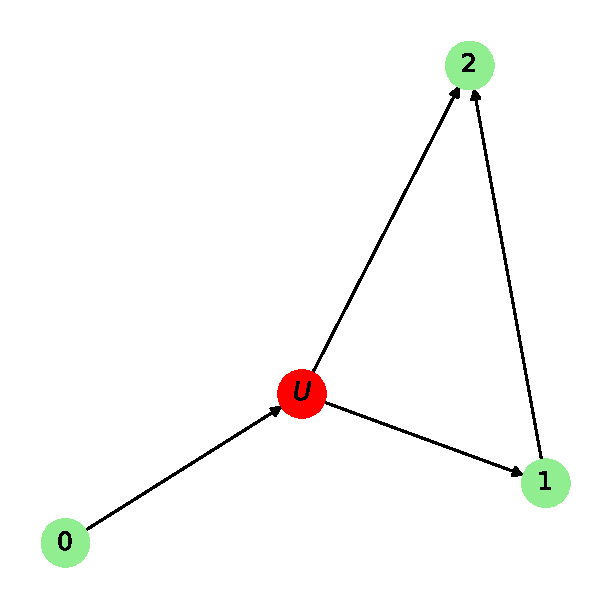
\includegraphics[width=\linewidth]{figures/ND examples/Hidden nodes/graph example w hidden.pdf}
        \caption{}
        \label{subfig:hidden nodes example unobserved}
    \end{subfigure}
    %
    \begin{subfigure}[t]{0.49\textwidth}
        \centering
        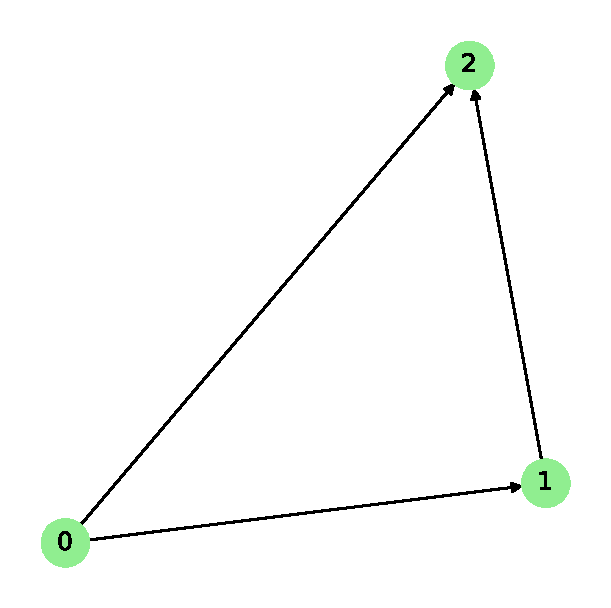
\includegraphics[width=\linewidth]{figures/ND examples/Hidden nodes/graph example wo hidden.pdf}
        \caption{}
        \label{subfig:hidden nodes example resulting graph}
    \end{subfigure}
    \caption{(a) An example of a causal structure depicted as a graph. When observing the network, only nodes $0$, $1$ and $2$ are observed/recorded. (b) The resulting inferred graph from observational data. Although this is not a complete picture of the true underlying dynamics of the system, if only the observed variables are of interest, this will be an equally proper representation of the system. Furthermore, in practice this means no further assumptions are made which can and can not be of desire. Namely, if prior information is accessible one might introduce new nodes in the inferred network.}
    \label{fig:hidden nodes example}
\end{figure}
With these initial comments, we proceed with the general setup and assumptions for network deconvolution based on observations.

\subsection{Setup and Assumptions}\label{subsec:Setup and assumptions}
Suppose a set of $d$ random variables $(X_i)$ is given i.e. a $d$-dimensional random vector $\boldsymbol X$. The method presented in this section aims to discover direct relationships between pairs $X_i$ and $X_j$ for $i\neq j$. \textcolor{blue}{These relationships will be presented by a directed graph as in the previous section or an undirected graph in case the causal direction is either unknown or such an assumption on direction is not plausible}. In particular, we shall let each random variable $X_i$ be represented by a vertex in a graph. We will later discuss a way of directing edges such that a causal network may be discovered i.e. a directed acyclic graph that may be used for inference.

The method proposed by \cite{Network-deconvolution-as-a-general-method-to-distinguish-direct-dependencies-in-networks} then works as follows. Given an observed matrix $G_{obs} \in \mathbb{R}^{d \times d}$ of similarities between each pair of variables, we shall deduce a matrix $G_{dir} \in \mathbb{R}^{d \times d}$ of direct similarities between each pair of random variables $X_i$ and $X_j$. \textcolor{blue}{In particular, we wish to filter out indirect effects which we will denote by $G_{dir}$ defined as effects between pairs of variables that is the result of effects propagating through other variables}. The measure of similarity, can in practice be any desired measure such as correlation or mutual information which we will focus on in this thesis. See \autoref{seq:Information measures and computation} for a further discussion on these two measures and \autoref{sec:Copula based network discovery} for how to obtain such a matrix. Note that the algorithm presented will in theory work for non-symmetric measures as well such as \textit{Interaction information}, \textit{Directed information} and \textit{Normalized information}.

\begin{figure}[ht]
    \centering
    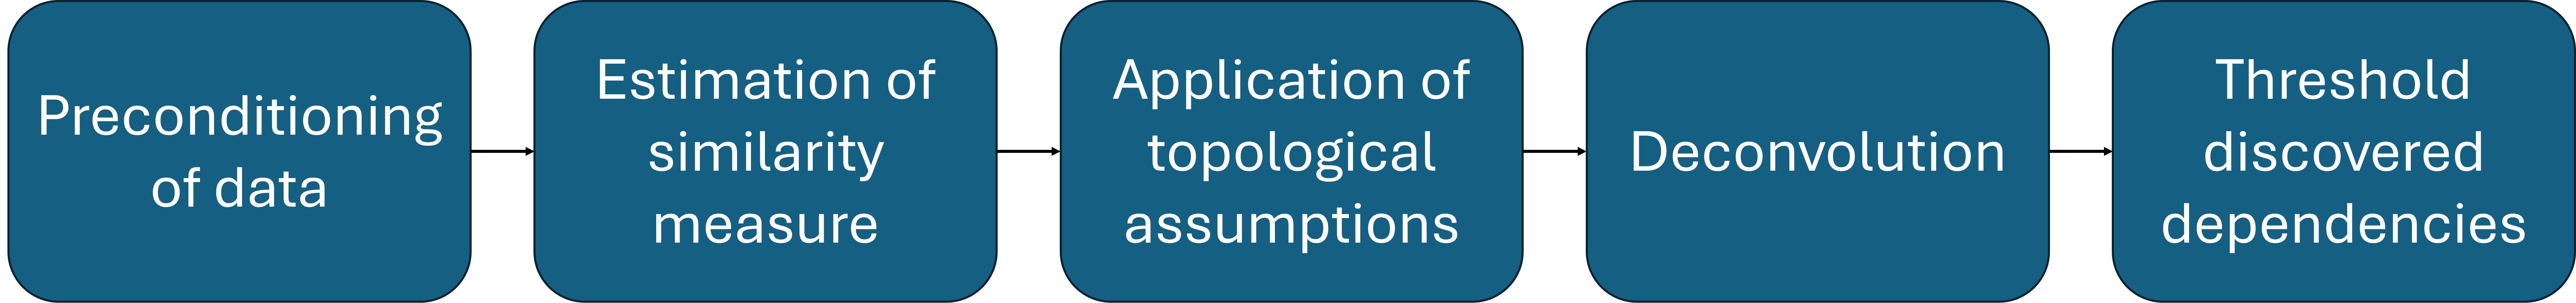
\includegraphics[width = \linewidth]{figures/Framework overview.png}
    \caption{On overview of the methodology that we shall develop in this thesis. In particular, the estimation of mutual information - a possible measure of similarity - and deconvolution will be discussed in this section.}
    \label{fig:Framework overview}
\end{figure}

% \textcolor{red}{Illustration of how the algorithm works and purpose}

The (direct) network is then presented by the discovered $G_{dir}$ containing only the direct effects i.e. interaction between pairs of variables which can be viewed as weights on the edges of the complete graph with nodes representing the random variables. As we shall see in \autoref{subseq:Robustness to noise}, the algorithm is somewhat robust to noise in the sense that we can ensure accuracy depending on the level of noise observed present in $G_{obs}$ and on the norm chosen (from a certain, although rather general, set of norms). \textcolor{blue}{Namely, if $G_{obs}$ is subject to noise, we find a bound on how different the inferred directed effects can be to the true direct effects using different matrix norms to measure this difference}. \textcolor{blue}{This hints to that a threshold on the inferred weights on the edges of the network might be a good idea to remove small inferred effects}. This is further supported by the facts that often only the most influential variables are of importance when trying to control the process.

The first assumption is that the observed matrix of co-dependence $G_{obs}$ may be expressed as
\begin{equation}
    G_{obs} = G_{dir} + G_{indir}
\end{equation}
Namely, that the direct and indirect effects can be added together to get the total and thus observed interdependence between each pair of variables. Often, this is not the case as we shall see later on. However, the error made from this assumption and the ones to be presented seem to be small enough that the discovered network accurately resemble the true underlying network.

The second and final assumption is that the indirect effects $G_{indir}$ can be computed in terms of $G_{dir}$. Namely, that
\begin{equation}
    G_{indir} = G_{dir}^2 + G_{dir}^3 + \dots = \sum_{k = 2}^{\infty} G_{dir}^k
\end{equation}
i.e. that the observed \textit{information} exchanged on an edge $e_{ij}$ between nodes $X_i$ and $X_j$ is the sum of the second, third etc. order effects, each given by the information on the $n$-path (where $n$ is the order of the (diminishing) indirect effect) again assumed to be a sum of products. In other terms, the second order indirect effect between $X_i$ and $X_j$ (given as the $(i,j)$ element of $G_{dir}^2$) is the sum of products on edges $e_{ik}$ and $e_{kj}$ for all $k$
$$\left[G_{dir}^2\right]_{ij} = \sum_{k=1}^d e_{ik}\,e_{kj}$$
where $e_{ij}$ is the $(i,j)$ element of $G_{dir}$. This is of course not true in general. However, through error analysis in \autoref{subseq:Robustness to noise} and controlled examples in \autoref{chap:results} we shall see that this assumption is either true under some additional assumptions or only results in small numerical errors. Immediately, we observe that $e_{ii}$ is of interest in terms of its physical meaning. The co-dependence between a random variable and itself might be somewhat ambiguous or even undefined depending on the measure. Thus, the notion of (non-existing) edges $e_{ii}$ will be of interest later on when using the method on controlled cases. We note that in $G_{obs}$ we shall in general set these elements to $0$.

Thus, from the above assumptions, it follows that we can express $G_{obs}$ as
\begin{equation}\label{eq:Network Informaiton Convolution}
    G_{obs} = G_{dir} + G_{dir}^2 + G_{dir}^3 + \dots = G_{dir} + G_{dir} \, G_{obs}
\end{equation}
Clearly, such a $G_{dir}$ must have spectral radius at most $1$ as otherwise, the above sum diverges and thus $G_{obs}$ will not exist. I.e. $\rho\left(G_{dir}\right) < 1$, where $\rho\left(\cdot\right)$ denotes the spectral radius. Thus, assuming convergence we can rewrite the infinite series as
\begin{equation}\label{eq:Gobs from Gdir}
    G_{obs} = G_{dir} \left(I - G_{dir}\right)^{-1}
\end{equation}
Multiplying the above by $\left(I - G_{dir}\right)$ from the right and moving around terms, it immediately follows that
\begin{equation}\label{eq:partial result on relation G_obs and G_dir}
    G_{obs} = G_{dir}\left(I + G_{obs}\right)
\end{equation}
Thus, if we can show that $-1 \not\in \sigma\left(G_{obs}\right)$ (where $\sigma \left(\cdot\right)$ denotes the spectrum of an operator), we can isolate $G_{dir}$. Namely, we need $-1$ to not be an eigenvalue of $G_{obs}$. This is indeed true under the assumption that $\rho\left(G_{dir}\right) < 1$. In particular, assume that $(\lambda, v)$ is an eigenpair of $G_{dir}$. Then, by assumption $\left|\lambda\right| < 1$ and by \autoref{eq:Network Informaiton Convolution}:
$$G_{obs}\, v = \sum_{k=1}^\infty G_{dir}^k v = \sum_{k=1}^\infty \lambda^k v = \frac{\lambda}{1-\lambda} v$$
where we used that $v$ is an eigenvector of $G_{dir}$ and the geometric series converges as $\left|\lambda\right| < 1$. In particular, $\left(\frac{\lambda}{ 1 - \lambda},\, v\right)$ is an eigenpair of $G_{obs}$. In \autoref{app:Jordan normal form of infinite matrix sum}, we show that $\lambda$ is an eigenvalue of $G_{dir}$ if and only if $\frac{\lambda}{1 - \lambda}$ is an eigenvalue of $G_{obs}$ i.e. there is a bijection between the eigenvalues of $G_{dir}$ and $G_{obs}$. Thus, as the spectral radius of $G_{dir}$ is less than one such that $\lambda \in (-1,1)$, we conclude that $\sigma\left(G_{obs}\right) \subset \left(-\frac{1}{2},\, \infty\right)$. Hence, $-1 \not\in \sigma \left(G_{obs}\right)$ and $G_{dir}$ can easily be isolated in \autoref{eq:partial result on relation G_obs and G_dir} as 
\begin{equation}\label{eq:Gdir from Gobs}
    G_{dir} = G_{obs} \left(I + G_{obs}\right)^{-1}
\end{equation}
We note that from the above, we have that $G_{obs}$ is a result of a $G_{dir}$ only if the smallest eigenvalue of $G_{obs}$ is larger than $-1/2$.

Furthermore, if the measure of dependence between pairs of variables is symmetric, then so is $G_{obs}$ and hence diagonalizable by some orthogonal matrix $U$ (such that $U^T = U^{-1}$) and diagonal matrix $\Lambda_{obs}$ such that $G_{obs} = U \Lambda_{obs} U^T$ (with the columns of $U$ being right eigenvectors of $G_{obs}$). This follows from the fact that any real symmetric matrix is diagonalizable. It follows that $G_{dir}$ can be expressed in the following simple way (which is useful for computational efficiency)
\begin{align*}
    G_{dir} &= U \Lambda_{obs} U^T \left(I + U \Lambda_{obs} U^T\right)^{-1}\\
    & = U \Lambda_{obs} U^T \left(U U^T + U \Lambda_{obs} U^T\right)^{-1}\\
    & = U \Lambda_{obs} U^T \left(U \left(I + \Lambda_{obs}\right) U^T\right)^{-1}\\
    & = U \Lambda_{obs} U^T U \left(I + \Lambda_{obs}\right)^{-1} U^T\\
    & = U \Lambda_{obs} \left(I + \Lambda_{obs}\right)^{-1} U^T\\
    & = U \Lambda_{dir} U^T
\end{align*}
where $\Lambda_{dir} = \Lambda_{obs} \left(I + \Lambda_{obs}\right)^{-1}$ is also a diagonal matrix, with elements corresponding to the inverse of the mapping $\lambda \mapsto \frac{\lambda}{1 - \lambda}$.

As we shall later use some assumptions regarding causality leading $G_{obs}$ to be a triangular matrix, we shall investigate the properties of the resulting $G_{dir}$. Namely, in the following, we show that given the existence of $G_{dir}$ (with necessary and sufficient conditions on $G_{obs}$ as given above), $G_{obs}$ is triangular if and only if $G_{dir}$ is triangular. Thus, by directing the observed similarity (by removing half the edge weights in $G_{obs}$), we also infer a directed graph $G_{dir}$.

Clearly, if $G_{dir}$ is triangular, so are the powers $G_{dir}^i$ for all $i\in\mathbb{N}$ and hence if the infinite sum $\sum_{i=1}^{\infty} G_{dir}^{i}$ converges, $G_{obs}$ is triangular as well.

To show the other way, assume that $G_{obs}$ is triangular and is the result of a $G_{dir}$ with spectral radius smaller than $1$. By \autoref{eq:Gdir from Gobs}, $G_{dir}$ is triangular if the inverse of $I + G_{obs}$ is triangular (upper triangular if $G_{obs}$ is also upper triangular and similarly for lower triangular). This is indeed the case as in general, the inverse of a triangular matrix is also triangular provided that the diagonal elements are non-zero.
% Later, we will set the diagonal of $G_{obs}$ to be $0$ (\autoref{eq:Gobs matrix}).
Note that  $ I + G_{obs}$ is never $0$ in the diagonal, as $-1/2$ is the smallest possible eigenvalue of $G_{obs}$ and hence smallest diagonal element. A simple proof is as follows. Assume without loss of generality, that a matrix $T$ is upper triangular. Let $D$ be the diagonal elements of $T$ and $T_u$ be the remaining strictly upper triangular part of $T$ such that $T = D + T_{u}$. Then, assuming that $D$ has non-zero diagonal elements, $T = D \left(I + D^{-1}T_u\right)$. Therefore,
\begin{align*}
    T^{-1} & = \left(I + D^{-1}T_u\right)^{-1} D^{-1}               \\
           & = \sum_{i=0}^\infty \left(- D^{-1} T_u\right)^i D^{-1}\\
           & = \sum_{i=0}^{d-1} \left(- D^{-1} T_u\right)^i D^{-1}
\end{align*}
which is clearly also upper triangular. The second and final equality follows from $T_u$ being strictly upper triangular and thus nilpotent such that $\sigma\left(-D^{-1} T_u\right) = \{0\}$ and $T_u^d = 0$. We conclude that $G_{obs}$ is triangular if and only if $G_{dir}$ is (under the assumption $G_{dir}$ exists and $G_{obs}$).

Finally, before discussing the implementation and analyzing the algorithm both analytically and through examples, we will take a closer look at the similarity measures that are to be used with this method and that in the end will make up the matrix $G_{obs}$. Namely, \textit{mutual information} and \textit{correlation}.


\section{Information Measures and Computation}\label{seq:Information measures and computation}
In this section we discuss two measures that can be used to construct the matrices of codependency from the previous section. Namely, we shall touch on correlation and discuss what one might choose to call Copula-based entropy. However, before discussing Copula entropy (CE) we first need to define what a copula is.

\subsection{Copula}
Given a set of $d$ random variables $X_1,\dots, X_d$, a copula is loosely speaking a distribution function with domain $[0,1]^d$ incorporating the dependence structure between the random variables. Given a joint distribution function $F$ for $\left(X_1,\dots, X_d\right)$ and (invertible) marginals $F_1,\dots,F_d$ we define a copula $C$ as
\begin{align*}
    F(x_1,\dots,x_d) & = \mathbb{P}\left(X_1\leq x_1,\dots, X_d\leq x_d\right)                                                                 \\
                     & = \mathbb{P}\left(F_1\left(X_1\right)\leq F_1\left(x_1\right),\dots, F_d\left(X_d\right)\leq F_d\left(x_d\right)\right) \\
                     & = C\left(F_1\left(x_1\right),\dots,F_d\left(x_d\right)\right)
\end{align*}
Letting $u_i = F_i\left(x_i\right) \in [0,1]$ it is clear that $C$ is a distribution function as described above \cite{Copula-handbook}. Furthermore, it follows that the marginals of $C$ are uniform as $F_i\left(X_i\right)$ is uniformly distributed. We thus define a copula in probabilistic terms as
\begin{definition}[Copula]\label{def:copula}
    A function $C:[0,1]^d \to [0,1]$ is called a copula if it has uniform marginals and is a distribution function for a $d$-dimensional random vector $\mathbf{X}$.
\end{definition}
An important and fundamental theorem of copulas for especially continuous random variables where the marginals are also continuous functions is stated by Sklar:
\begin{theorem}[Sklar's theorem] \label{thm: Sklar}
    For a random vector $\boldsymbol X$ with CDF $F$ and univariate marginal CDFs $F_1, \dots, F_d$. There exists a copula $C$ such that
    \begin{equation}\label{eq:sklar}
        F(x_1,\dots,x_d) = C(F_1(x_1), \dots, F_d(x_d))
    \end{equation}
    If $X$ is continuous, $C$ is unique; otherwise $C$ is uniquely determined on the Cartesian product of the ranges of distribution functions $F_i$, $\prod \text{Ran}\left(F_i\right)$.
\end{theorem}
Note that the last statement for non-continuous random variables can be made unique by instead using subcopulas, a generalization of copulas with domain $I$ only a subdomain of the unit hypercube $\mathbb{I}^d = [0,1]^d$ containing all faces of the unit hyper cube. However, there are infinitely many ways of extending such a subcopula to a copula $C$\cite{Copula-modeling-for-discrete-random-vectors}. In our case, this means that for discrete and/or mixed variables, we will later have to work around this non-uniqueness when calculating mutual information. The example made by Geenens\cite{Copula-modeling-for-discrete-random-vectors} is a bivariate random vector of independent variables $X \sim \text{Bern}\left(\pi_X\right)$ and $Y\sim \text{Bern}\left(\pi_Y\right)$. The support of $F_X$ and $F_Y$ is then $\{0, 1-\pi_X\}$ and $\{0, 1-\pi_Y\}$ respectively. Due to the restriction on the boundary of the unit square, the only unique point of a copula $C$ is then $(1-\pi_X, 1-\pi_Y)$, and by independence we must have
$$C\left(1-\pi_X, 1-\pi_Y\right) = (1-\pi_X)( 1-\pi_Y)$$
Geenens then proceed to define an uncountable set of copulas that fulfill the above criterion which further illustrates that the basic concepts of copulas are not well suited for discrete random vectors. Note that in the article it is however argued how one can extend the concept to a more general concept that works for mixed variables.

From \autoref{eq:sklar} we see that a copula is thus simply just a function that \textit{couples} the marginals of a random vector to the joint distribution. The following corollary follows immediately
\begin{corollary}[Coordinate transformation] \label{coro: Coordinate transformation}
    Under the assumptions of \autoref{thm: Sklar}, given any set $(T_1, \dots, T_d)$ of strictly increasing functions, if $C$ is a copula of $(X_1,\dots, X_d)$ then it is also a copula of $(T_1(X_1), \dots, T_d(X_d))$.
\end{corollary}
\begin{proof}
    Suppose $(X_1 , \dots , X_d)$ permits a copula $C$ and let $T_i$ be given as stated. Consider coordinate wise the result of the transformation $Y_i = T_i(X_i)$ and consider the CDF $F_{Y_i}(y_i)$
    \begin{align*}
        F_{Y_i}(y_i) & = \mathbb{P}\left(Y_i \leq y_i\right)                      \\
                     & = \mathbb{P}\left(T_i^{-1}(Y_i) \leq T_i^{-1}(y_i)\right)  \\
                     & = \mathbb{P}\left(X_i \leq T_i^{-1}\left(y_i\right)\right) \\
                     & = F_{X_i}\left(T_i^{-1}\left(y_i\right)\right)
    \end{align*}
    The above is easily generalized for a joint distribution as well. Thus, by the existence of a copula $C$ for $\boldsymbol{X}$
    \begin{align*}
        F_{\boldsymbol Y}(y_1, \dots, y_d) & = F_{\boldsymbol X} \left(T_1^{-1}\left(y_1\right),\dots , T_d^{-1}\left(y_d\right)\right)   \\
                                           & = C\left( F_{X_1}(T_1^{-1}\left(y_1\right)), \dots, F_{X_d}(T_d^{-1}\left(y_d\right))\right) \\
                                           & = C\left( F_{Y_1}(y_1), \dots, F_{Y_d}(y_d)\right)
    \end{align*}
    where Sklar's theorem have been used for the second equality. The above shows that $C$ is indeed also a copula for $\boldsymbol Y = \left(T_1(X_1), \dots, T_d(X_d)\right)$.
\end{proof}
The above corollary is actually equivalent with a seemingly stronger statement and follows easily
\begin{proposition}
    Since $T_i$ is strictly increasing, the inverse $T_i^{-1}$ exists and is also strictly increasing. Thus, the above implication is bidirectional and hence for strictly increasing functions $T_i$, $C$ is a copula of $\left(X_1,\dots,X_d\right)$ if and only if it is a copula of $\left(T_1(X_1),\dots, T_d(X_d)\right)$.
\end{proposition}












\subsection{Mutual Information and Copula Entropy}
In this section we introduce copula entropy as done in \cite{Nonparametric-copula-entropy-and-network-deconvolution-method-for-causal-discovery-in-complex-manufacturing-systems} and see how it actually is equal to the well known mutual information (multiplied by $-1$) and hence as a corollary that mutual information is independent of marginals. The name comes from the general definition of (differential) entropy as we shall see shortly. However, first we define mutual information between a set of random variables
\textcolor{blue}{
    \begin{definition}[Mutual information]\label{def:mutual information}
        For a random vector $\boldsymbol{X} = \{X_i\}$, we define the mutual information as
        $$I(\boldsymbol{X}) = \mathbb{E}\left[\log_b \left(\frac{f(\boldsymbol X)}{\prod_i f_i (X_i)}\right)\right]$$
        % $$I(\boldsymbol{X}) = \sum_{\boldsymbol{x} \in \mathcal{X}} f(\boldsymbol{x}) \, \log_b\left(\frac{f(\boldsymbol{x})}{\prod_{i} f_i\left(x_i\right)}\right)$$
        where $f$ is the joint density function with marginals $f_i$ of the random vector $\boldsymbol{X}$.
        % If $\boldsymbol X$ is discrete and $f$ is the joint probability mass function with marginals $f_i$. Similarly, for continuous random vectors with $f$ the joint probability density function we define
        % $$I(\boldsymbol{X}) = \int_{\mathcal{X}} f(\boldsymbol{x}) \, \log_b\left(\frac{f(\boldsymbol{x})}{\prod_{i} f_i\left(x_i\right)}\right)\, d\boldsymbol{x}$$
        The base of the logarithm $b$ is often chosen to be $2$, $e$ or $10$ although the choice is unimportant as all logarithms are equivalent up to a scaling factor.
    \end{definition}
}
We note that later on, as the choice of $b$ will result in a scaling of $G_{obs}$, but we will also introduce a scaling parameter $\alpha$ for $G_{obs}$ to both ensure the convergence of the algorithm and to control higher order effects, we shall in general choose $b = e$.

An important property of mutual information is that the continuous version is the limit of the discrete mutual information for random (continuous) vector discretized as the mesh size goes to zero i.e. recovering the continuity of the random vector. This is discussed in \autoref{subsec:limit entropy and MI}. For now, we proceed with the definition of (joint) entropy for both discrete and continuous random vectors.
\textcolor{blue}{
    \begin{definition}[Entropy]\label{def:entropy}
        The (joint) entropy of a random vector $\boldsymbol{X}$ is defined as
        % $$H\left(\boldsymbol{X}\right) = - \sum_{\boldsymbol{x}\in \mathcal{X}} f(\boldsymbol{x}) \, \log_b f(\boldsymbol{x})$$
        $$H\left(\boldsymbol{X}\right) = - \mathbb{E}\left[\log_b f(\boldsymbol X)\right]$$
        In case of a discrete random vector, this is called the Shannon entropy while for continuous random vectors, this is called differential entropy and is often denoted as $h\left(\boldsymbol X\right)$ instead of $H\left(\boldsymbol X\right)$.
    \end{definition}
}
% And likewise for continuous random vectors, which we name differential entropy
% \begin{definition}[Differential entropy]\label{def:differential entropy}
%     The (joint) differential entropy defined for a continuous random vector $\boldsymbol{X}$ is defined as
%     $$h(\boldsymbol{X}) = - \int_{\mathcal{X}} f\left(\boldsymbol{x}\right) \, \log_b f\left(\boldsymbol{x}\right) \, d\boldsymbol{x}$$
% \end{definition}
We note the need for two separate notations of entropy as differential entropy is not the limit of Shannon entropy in the way mutual information is. Again, this is further discussed in \autoref{subsec:limit entropy and MI}.
% However, they are both equal to the expectation $\mathbb{E}\left(\log f\left(\boldsymbol X\right)\right)$.

Before discussing copula entropy (CE), we note a very useful relation between entropy and mutual information. Indeed, we shall later use this to show that mutual information in the continuous version is the limit of the discretization.
\begin{lemma}[Mutual information and entropy relation]\label{lemma:mutual information and entropy relation}
    For a continuous random vector $\boldsymbol{X}$, the (joint) mutual information $I\left(\boldsymbol{X}\right)$ can be decomposed into a sum of differential entropies as
    $$I\left(\boldsymbol{X}\right) = \sum_{i=1}^{d} h(X_i) - h\left(\boldsymbol{X}\right)$$
    where $d$ is the dimension of $\boldsymbol{X}$. The same is true for discrete variables but with entropy $H$ instead of differential entropy $h$.
\end{lemma}
\textcolor{blue}{\begin{proof}
        This follows immediately from the definition of mutual information and entropy:
        $$\mathbb{E}\left[\log_b \frac{f\left(\boldsymbol X\right)}{\prod_i f_i\left(X_i\right)}\right] = \mathbb{E}\left[\log_b f\left(\boldsymbol X\right) \right] - \sum_i \mathbb{E}\left[\log_b f_i \left(X_i\right)\right]$$
        % The proof is identical for discrete and continuous random vectors. Hence, we only show the proof in the continuous case. By direct computation
        % \begin{align*}
        %     I\left(\boldsymbol{X}\right) & = \int_{\mathcal{X}} f\left(\boldsymbol{x}\right) \, \log_b f\left(\boldsymbol{x}\right) \, d\boldsymbol{x} - \sum_{i = 1}^{d} \int_{\mathcal{X}} f\left(\boldsymbol{x}\right) \, \log_b f_i\left(x_i\right) \, d\boldsymbol{x} \\
        %                                  & = \int_{\mathcal{X}} f\left(\boldsymbol{x}\right) \, \log_b f\left(\boldsymbol{x}\right) \, d\boldsymbol{x} - \sum_{i = 1}^{d} \int_{\mathcal{X}_i} f_i\left(\boldsymbol{x}\right) \, \log_b f_i\left(x_i\right) \, d x_i       \\
        %                                  & = \sum_{i=1}^{d} h\left(X_i\right) - h\left(\boldsymbol{X}\right)
        % \end{align*}
    \end{proof}}
With the definitions of mutual information and entropy we are finally ready to introduce copula entropy.
\begin{definition}[Copula entropy]\label{def:copula entropy}
    For a continuous random vector $\boldsymbol{X}$ with a uniquely defined copula $C$, and copula density $c$, we define the copula entropy $CE$ of $\boldsymbol{X}$ as
    $$CE\left(\boldsymbol{X}\right) = h\left(\boldsymbol U\right)$$
    where $\boldsymbol U$ has density $c$. In particular,
    $$CE\left(\boldsymbol{X}\right) = - \mathbb{E}\left[\log_b c \left(\boldsymbol U\right)\right]$$
    % $$CE\left(\boldsymbol{X}\right) = - \int_{[0,1]^d} c\left(\mathbf{u}\right) \, \log_b c\left(\mathbf{u}\right) \, d\mathbf{u}$$
\end{definition}
As stated above, copula entropy is actually equal to the negative mutual information which we state as a theorem
\begin{theorem}[Equality of Copula entropy]\label{thm:copula entropy equals mutual information}
    For a continuous random vector $\boldsymbol{X}$, the copula entropy $CE$ is equal to the negative joint mutual information of $\boldsymbol{X}$
    $$CE\left(\boldsymbol{X}\right) = - I\left(\boldsymbol{X}\right)$$
\end{theorem}
\begin{proof}
    By \autoref{thm: Sklar}, letting $x_i = F_i^{-1}\left(u_i\right)$, we can relate the copula density to the joint density of $\boldsymbol{X}$ and its marginals
    \begin{align*}
        c(u_1,\dots , u_n) & = \frac{\partial}{\partial \mathbf{u}} C(u_1,\dots,u_n)                                                                                                                   \\
                           & = \frac{\partial}{\partial \mathbf{u}} F\left(F_1^{-1}\left(u_1\right), \dots, F_n^{-1}\left(u_n\right)\right)                                                            \\
                           & = f\left(F_1^{-1}\left(u_1\right),\dots, F_1^{-1}\left(u_n\right)\right) \frac{1}{f_1\left(F_1^{-1}\left(u_1\right)\right)\dots f_n\left(F_1^{-1}\left(u_d\right)\right)}
    \end{align*}
    It follows directly that
    \begin{align*}
        -CE\left(\boldsymbol{X}\right) & = \int_{[0,1]^d} c\left(\boldsymbol{u}\right) \log c\left(\boldsymbol{u}\right) \, d\boldsymbol{u}                                                                                                                        \\
                                       & =  \int_{\mathcal{X}} \frac{f(\boldsymbol{x})}{\prod_{i=1}^{d} f_i\left(x_i\right)} \log\left(\frac{f(\boldsymbol{x})}{\prod_{i=1}^{d} f_i\left(x_i\right)}\right) \prod_{i=1}^{d} f_i\left(x_i\right) \, d\boldsymbol{x} \\
                                       & = \int_{\mathcal{X}} f(\boldsymbol{x}) \log\left(\frac{f(\boldsymbol{x})}{\prod_{i=1}^{d} f_i\left(x_i\right)}\right) \, d\boldsymbol{x}                                                                                  \\
                                       & = I\left(\boldsymbol{X}\right)
    \end{align*}
    where $\mathcal{X}$ is the domain of the random variable $\boldsymbol X$ and the third equality follows from a change of variables with the trivial substitution $u_i = F_i(x_i)$ such that $du_i = f_i(x_i)\,dx_i$. This concludes the proof.
\end{proof}
Finally, before moving on to correlation as a measure of similarity, we discuss what happens in the limit of mutual information and entropy as we shall later need this as arguments for numerical stability.


\subsection{Entropy and Mutual Information in the Limit}\label{subsec:limit entropy and MI}
In this section, we shall discuss the differences between entropy and differential entropy and observe how this difference cancels when computing mutual information. In fact, we shall see that mutual information defined for continuous random vectors is the limit of the discrete version which will be useful later when implementing the algorithm.

First, although one may think differential entropy is the limit of (discrete) entropy, this is not the case. Namely, consider the support of $f(x)$ (here assumed to be the entire real line) binned into intervals i.e. a discretization of the continuous random variable $X$, which we shall denote $X^{\Delta}$. To make notation simpler, we shall bin into equal-sized intervals of width $\Delta$. Then, for each interval $[i\Delta, (i+1)\Delta)$ for $i \in \mathbb{Z}$, there exists an $x_i$ such that the probability mass on this interval is represented by this $x_i$:
\textcolor{blue}{
    \begin{equation}\label{eq:one dim discretization}
        \mathbb{P}\left(X^{\Delta} = x_i\right) = f(x_i) \Delta = \int_{i\Delta}^{(i+1)\Delta} f(x) \, dx
    \end{equation}
}
Clearly, this discretization is a valid distribution as
$$\sum_{i\in\mathbb{Z}} f(x_i) \Delta = \int_{\mathbb{R}} f(x) \, dx = 1$$
and in the limit, as $\Delta \to 0$ we recover the original distribution $f(x)$. However, if we try to calculate the entropy of this discretization, denoted by $H^{\Delta}$, we get a diverging limit
\begin{align*}
    H^{\Delta} & = -\sum_{i\in\mathbb{Z}} f(x_i) \Delta \log{f(x_i) \Delta}                                             \\
               & = -\sum_{i\in\mathbb{Z}} f(x_i) \Delta \log{f(x_i)} - \sum_{i\in\mathbb{Z}} f(x_i) \Delta \log{\Delta} \\
               & = -\sum_{i\in\mathbb{Z}} f(x_i) \Delta \log{f(x_i)} - \log{\Delta}
\end{align*}
Clearly, the first term in the above expression converges to the differential entropy $h\left(X\right)$ as $\Delta \to 0$ whereas $\log{\Delta} \to - \infty$ i.e. the expression diverges altogether when differential entropy is well-defined.

A similar argument for the joint entropy between the discretization of $X_1$ and $X_2$ (and in principle to any number of dimensions), denoted by $H^{\Delta}_{12}$, results in
$$H^{\Delta}_{12} = -\sum_{i,j \in \mathbb{Z}} f\left(x_1^{(i)}, x_2^{(j)}\right) \Delta_1 \Delta_2 \log{f\left(x_1^{(i)}, x_2^{(j)}\right)} - \log{\Delta_1} - \log{\Delta_2}$$
where $x_1^{(i)}\in[i\Delta_1, (i+1)\Delta_1)$ and $x_2^{(j)}\in [j\Delta_2, (j+1)\Delta_2)$ are defined such that
$$f\left(x_1^{(i)}, x_2^{(j)}\right)\Delta_1 \Delta_2 = \int_{j\Delta_2}^{(j+1)\Delta_2}\int_{i\Delta_1}^{(i+1)\Delta_1} f(x_1,x_2) \, dx_1 dx_2,\quad \forall i,j\in\mathbb{Z}$$
Note that clearly $\left(x_1^{(i)},x_2^{(j)}\right)$ exists for all $i,j\in \mathbb{Z}$. Again, the joint entropy diverges however, when computing the mutual information, we see that the diverging terms cancel. Namely, from \autoref{lemma:mutual information and entropy relation}
\begin{align*}
    I^{\Delta}_{12} & = H^{\Delta}_1 + H^{\Delta}_2 - H^{\Delta}_{12}                                                                                                                                                                      \\
                    & = -\sum_{i\in\mathbb{Z}} f_1\left(\tilde{x}_1^{(i)}\right) \Delta_1 \log{f_1\left(\tilde{x}_1^{(i)}\right)} - \log{\Delta_1}                                                                                         \\
                    & \quad - \sum_{j\in\mathbb{Z}} f_2\left(\tilde{x}_2^{(j)}\right) \Delta_2 \log{f_2\left(\tilde{x}_2^{(j)}\right)} - \log{\Delta_2}                                                                                    \\
                    & \quad + \sum_{i,j\in\mathbb{Z}} f\left(x_1^{(i)},x_2^{(j)}\right) \Delta_1 \Delta_2 \log{f\left(x_1^{(i)},x_2^{(j)}\right)} + \log{\Delta_1 \Delta_2}                                                                \\
                    & =-\sum_{i\in\mathbb{Z}} f_1\left(\tilde{x}_1^{(i)}\right) \log{f_1\left(\tilde{x}_1^{(i)}\right)}\Delta_1 - \sum_{j\in\mathbb{Z}} f_2\left(\tilde{x}_2^{(j)}\right)  \log{f_2\left(\tilde{x}_2^{(j)}\right)}\Delta_2 \\
                    & \quad +\sum_{i,j\in\mathbb{Z}} f\left(x_1^{(i)},x_2^{(j)}\right) \log{f\left(x_1^{(i)},x_2^{(j)}\right)} \Delta_1 \Delta_2                                                                                           \\
                    & \to h(X_1) + h(X_2) - h(X_1,X_2)\; \text{as}\; \Delta_1,\Delta_2 \to 0
\end{align*}
Thus, the limit of the mutual information for discrete random variables is indeed the mutual information defined for continuous random variables and can be computed either as the limit of discretizing the probability density function and then computing entropies or just using the initial definition for (discrete) mutual information in \autoref{def:mutual information}. In particular, mutual information for discrete and random variables are comparable such that it makes sense define mutual information between mixed random variables. For a more rigorous treatment of this, we refer to \cite{Estimating_Mutual_Information_for_Discrete-Continuous_Mixtures} where they define mutual information between discrete and continuous random variables from a measure theoretical point of view.


Before continuing, we discuss the case where $X_1$ is equal to $X_2$. In this case, discretizing with a common $\Delta$ we have that
$$f\left(x_1^{(i)}, x_2^{(j)}\right)\Delta^2 = \int_{j\Delta}^{(j+1)\Delta}\int_{i\Delta}^{(i+1)\Delta} f(x_1,x_2) \, dx_1 dx_2,\quad \forall i,j\in\mathbb{Z}$$
Clearly, the above integral is $0$ for $i\neq j$. Although $f(x_1,x_2)$ is not well-defined in the usual functional sense, extending to distribution, we might write $f(x_1,x_2) = f(x_2 | x_1) f(x_1)$. In terms of distributions, it works to put $f(x_2 | x_1) = \delta(x_2 - x_1)$ where $\delta$ is the \textit{Dirac delta} distribution, as then $\int_{\mathbb{R}} f(x_1,x_2) \, dx_2 = f(x_1)$ and $f(x_1, x_2)$ is "$0$" when $x_1 \neq x_2$. I.e. the marginals and probability mass are correct. Then, when calculating the above integral, we get that
\begin{align*}
    f\left(x_1^{(i)}, x_1^{(i)}\right)\Delta^2 & = \int_{i\Delta}^{(i+1)\Delta}\int_{i\Delta}^{(i+1)\Delta} f(x_1,x_2) \, dx_1 dx_2 \\
                                               & = \int_{i\Delta}^{(i+1)\Delta} f\left(x_1\right)\, dx_1                            \\
                                               & = f\left(\tilde{x}_1^{(i)}\right)\Delta
\end{align*}
Thus, when calculating $I^{\Delta}$ for two identical variables, we obtain
\begin{align*}
    I^{\Delta} & = -\sum_{i\in\mathbb{Z}} f\left(\tilde{x}_1^{(i)}\right) \log{f\left(\tilde{x}_1^{(i)}\right)}\Delta - \sum_{j\in\mathbb{Z}} f\left(\tilde{x}_2^{(j)}\right)  \log{f\left(\tilde{x}_2^{(j)}\right)}\Delta \\
               & \quad + \sum_{i\in\mathbb{Z}} f\left(\tilde{x}_1^{(i)}\right) \log{f\left(\tilde{x}_1^{(i)}\right)}\Delta - \log \Delta                                                                                   \\
               & \to \infty \;\text{as}\; \Delta \to 0
\end{align*}
Thus in practice, it would not make much sense to compare equal variables or even a random vector only defined on a lower dimensional manifold as we would get an infinite copula entropy.





\subsection{Correlation}
At this point, we have a good understanding of copula entropy/mutual information for calculations later on. However, another typical measure of similarity is correlation which is easily estimated from sample data. However, in this section we show that in general, we can not compute the correlation coefficient from a copula which we saw above is the case for mutual information. Namely, given a copula $C$ for some set of random variables $\{X_i\}_{i\in I}$ indexed by finite $I$, one can not calculate $\rho$ between any pair $(X_i ,X_j)$, $i\neq j$ from the copula. This is easily shown by the following argument.

First, note that from \autoref{coro: Coordinate transformation}, $C$ is also a copula for $Z_i \coloneq \left( X_i - \mu_i\right) / \sigma_i$ for $i \in I$ where $\mu_i = \mathbb{E}[X_i]$ and $\sigma_i = \sqrt{\text{Var} \, X_i}$ (assuming that these exist). Clearly, the correlation coefficient for $Z_i$ and $Z_j$ is the same as between $X_i$ and $X_j$. We thus proceed trying to calculate the correlation between any pair $Z_i$ and $Z_j$.
\begin{equation}\label{eq:corr from copula}
    \begin{split}
        \rho_{ij} & = \int\int_{\mathbb{R}^2} z_i z_j f_{ij}(z_i,z_j) \, dz_i \, dz_j                       \\
                  & = \int\int_{[0,1]^2} F_i^{-1}(u_i) \, F_j^{-1}(u_j) \, c_{ij}(u_i, u_j) \, du_i \, du_j
    \end{split}
\end{equation}
where $c_{ij}$ density version of the copula defined for $X_i$ and $X_j$ and $F_i$ and $F_j$ are the marginals of $Z_i$ and $Z_j$ with mean $0$ and variance $1$. From the above, it is then clear for a fixed, non-constant copula $C$, the correlation depends on the marginals of $X_i$ and $X_j$. Also, we see that a constant copula density (only admissible if $c \equiv 1$ on $[0,1]^2$ and $0$ elsewhere) always results in $\rho_{ij} = 0$ as
$$\int_0^1 F^{-1}(u) \, du = \int_{\mathbb{R}} z f(z) \, dz = 0$$
where the final equality follows from the construction of $Z_i$.

Thus, we conclude that indeed mutual information and correlation are very different measures of codependency. Namely, mutual information does not depend on the marginal distributions whereas from \autoref{eq:corr from copula} we see that correlation does. Thus, it does not make much sense to introduce copulas in the setting of correlation albeit at this point we do not favor one measure above the other except if marginals should be insignificant to the network, copula entropy is preferred.






\section{Copula Based Network Discovery}\label{sec:Copula based network discovery}
In this section, we will present the general algorithm and discuss some of its properties regarding uncertainty and convergence. We will focus on using mutual information i.e. copula entropy as the measure of similarity but other measures such as correlation can be interchanged at will in the general algorithm.

By \autoref{thm:copula entropy equals mutual information} we can compute the mutual information from observed data from the copula. Namely, let $CE_{ij}$ denote the (pairwise) copula entropy of variables $X_i$ and $X_j$. We shall then set
\begin{equation}\label{eq:Gobs matrix}
    G_{obs} = \begin{bmatrix}
        0        & - CE_{12} & \dots  & - CE_{1n} \\
        -CE_{21} & 0         & \dots  & - CE_{2n} \\
        \vdots   & \vdots    & \ddots & \vdots    \\
        -CE_{n1} & -CE_{n2}  & \dots  & 0
    \end{bmatrix}
\end{equation}
where $n$ is the number of nodes in the graph i.e. random variables that we have observed. Notice that we have chosen the diagonal elements as $0$ since information between a random variable $X$ and itself is not really well-defined and when trying to compute this numerically, we observe diverging results as also discussed in the previous section. Furthermore, only the information that propagates through the network is of interest and so setting $0$ in the diagonal avoids a bias when deconvolving the information or any similarity in general. Especially for mutual information where the information between a variable and itself diverges to $\infty$ thus in the limit, from \autoref{eq:Gdir from Gobs}, we would get the identity matrix which does not tell us much about the direct dependencies.

\autoref{alg:Gobs1} then follows immediately from \autoref{eq:Gobs matrix}
\begin{algorithm}[H]
    \caption{$G_{obs}$ computation}\label{alg:Gobs1}
    \begin{algorithmic}
        \Require $n > 0$             \Comment{Number of variables}
        \State $G_{obs} \gets \boldsymbol 0$
        \For{$1\leq i , j \leq n\; | \; i\neq j$}
        \State Estimate $F_i$ and $F_j$ from $x_i^{\mathcal{D}}$ and $x_j^{\mathcal{D}}$
        \State $u_i^{\mathcal{D}} \gets F_i(x_i^{\mathcal{D}})$
        \State $u_j^{\mathcal{D}} \gets F_j(x_j^{\mathcal{D}})$
        \State Estimate $c_{ij}$ from $u_i^{\mathcal{D}}$ and $u_j^{\mathcal{D}}$
        \State Compute $NCE_{ij}$
        \State $\left[G_{obs}\right]_{ij} \gets -NCE_{ij}$
        \EndFor
        \State \Return $G_{obs}$
    \end{algorithmic}
\end{algorithm}
Namely, for each entry in $G_{obs}$, except for the diagonal elements, first estimate the cumulative distributions of $X_i$ and $X_j$ based on samples $x_i^{\mathcal{D}}$. Then, transform the samples by the estimated distribution function to obtain corresponding uniform samples. This may be done outside the loop to increase computational efficiency. From the paired samples $(x_i^{\mathcal{D}},x_j^{\mathcal{D}})$, estimate the copula density $c_{ij}$ and finally use this to compute the mutual information/copula entropy. Methods for estimating the densities and in continuation hereof the distribution functions are presented in \autoref{subsec:Mutual information estimation and KDE methods}. The negative copula entropy is then recorded in $(i,j)$ entry of $G_{obs}$. We note that the algorithm can be optimized for symmetric measures such as copula entropy itself, to only loop through $i<j$ and saving the computed entropy in the $(j,i)$ entry as well. Also, as copula entropy diverges as $X_i$ and $X_j$ are jointly distributed closer to a one-dimensional manifold, ideally there should be a check for such or the user should check the paired observations to exclude such variable combinations.

From \autoref{subsec:limit entropy and MI}, to calculate the (joint) copula entropy of a continuous random vector, we simply discretize the domain of each random variable and use the estimated copula density evaluated at these points to estimate the total copula entropy. Furthermore, if one or more elements of the random vector are mixed random variables, we choose the discrete events to be their own bins and discretize the rest or in the context of \autoref{alg:Gobs1} only estimate the distribution functions for the continuous component of the random variable. This works due to the copula entropy for continuous random variables being the limit of the discretization and as such, the copula entropy is well-defined for mixed random variables as well.

We continue with an example of how this discretization of a mixed random variable would work. Notice that we only have a discrete event (an atom) at $0$ as this resembles the observed behavior of the delays, although the example could be extended to more complex discrete distributions.



\begin{example}[Discrization of mixed random variable]\label{ex:discrization of mixed random variable}
    Let $X$ be a mixture of an atom in e.g. $0$ and an exponential with parameter $\lambda$ with proportions $p$ and $1-p$. Then, a discretization of $X$ is $0$ with probability mass $p$ and the remaining support $(0,\infty)$ discretized in some way with total probability mass $1-p$ and each bin having probability according to \autoref{eq:one dim discretization} scaled with $1-p$. If the bin size is a constant $\Delta$, then for the discretized variable $X^{\Delta}$, we have $\mathbb{P}\left(X^{\Delta} = 0\right) = p$ and $\mathbb{P}\left(X^{\Delta} = x_i\right) = (1-p) \exp{(-\lambda i \Delta)}\left(1- \exp(-\lambda \Delta)\right)$, where $x_i$ is given by
    $$x_i = i \Delta  + \frac{1}{\lambda} \left(\log \left( \lambda \Delta\right) - \log \left(1 - e^{-\lambda \Delta}\right)\right), \quad i \in \mathbb{N}_0$$
\end{example}











% \textcolor{red}{We shall see shortly that these (entropy continuous and discrete) are not the limit of each other (discrete to continuous) but when using MI it does not matter and even makes implemtaiton simpler}



\subsection{Network Deconvolution}
At this point, we have obtained a convolved matrix of information $G_{obs}$ and are ready to use \autoref{eq:Gdir from Gobs}. We present the original algorithm from \cite{Network-deconvolution-as-a-general-method-to-distinguish-direct-dependencies-in-networks} in the case $G_{obs}$ is symmetric and hence diagonalizable by an orthogonal matrix $U$. The original \texttt{Matlab} implementation was translated to \texttt{Python} and is summarized in the following pseudocode.
\begin{algorithm}[H]
    \caption{(ND) Network Deconvolution}\label{alg:ND}
    \begin{algorithmic}
        \Require $G_{obs}$, $\alpha$, $\beta$             %\Comment{Input observational matrix}
        % \For{$0\leq i < j < N$}
        \State $\left[G_{obs}\right]_{ii} \gets 0, \; \forall i\in \{1,\dots, d\}$                    \Comment{ensure zero-diagonal}
        % \State $Q_p \gets G_{[1-\alpha]}$
        \State $\left[G_{obs}\right]_{ij} \gets 0$, when $\left[G_{obs}\right]_{ij} < Q_{\alpha}\left(G_{obs}\right)$
        \State Compute eigendecomposition $U,\Lambda$ of $G_{obs}$
        \State $\lambda^+ \gets  \max{ \left( \lambda^{\text{max}},0 \right) }$
        \State $\lambda^- \gets \min{ \left( \lambda^{\text{min}},0 \right) }$
        \State $k^+ \gets \frac{1-\beta}{\beta} \lambda^+$
        \State $k^- \gets \frac{1+\beta}{\beta} \lambda^-$
        \State $c_s^{-1} \gets \max{\left( k^+, - k^- \right)}$
        \State $\hat{\Lambda} \gets \Lambda \left(c_s^{-1}I + \Lambda\right)^{-1}$
        \State \Return $U \hat{\Lambda} U^T$
        % \EndFor
    \end{algorithmic}
\end{algorithm}
where $Q_{\alpha} \left(G_{obs}\right)$ denotes the $\alpha$ quantile of the strictly upper (or lower due to symmetry) triangular part of $G_{obs}$. We note the two extra parameters $alpha$ and $\beta$ which we will discuss shortly. In particular, the paper contains conflicting information on how to find $\beta$ from how it is defined. Furthermore, they include some analysis on the robustness of the above deconvolution algorithm but only in a somewhat particular case and with some confusion on matrix norms and spectral radius. This analysis on robustness, we will extend and clarify in the following \autoref{subseq:Robustness to noise}.

From the definition of $Q_{\alpha}\left(G_{obs}\right)$ it is clear that the $\alpha$ parameter is a filter on the observed edges and is useful if one wants to filter out insignificant observations. However, in practice, as we will see, it is often not very influential except for large $\alpha$ (corresponding to many edges set to $0$) as small perturbations from e.g. imperfect calculations should not influence the results for fairly conditioned matrices as we shall observe in \autoref{sec:gaussian MI error}. Thus, setting $\alpha = 0$ retains all values in $G_{obs}$ after setting the diagonal equal to $0$. As a technical detail, we note that the \texttt{quantile} function from \texttt{NumPy} (v. 1.26.4) has been used to find this quantile as quantiles can be defined in many ways from a data set.

Finally, we note that the $\beta \in (0,1)$ parameter corresponds to a scaling of $G_{obs}$ such that the resulting spectral norm of $G_{dir}$ is $\beta$. From \autoref{alg:ND} it is seen that it serves as a regularization on the eigenvalues of $G_{obs}$ and although this is discussed in \cite{Network-deconvolution-as-a-general-method-to-distinguish-direct-dependencies-in-networks}, their results do not conform with their implementation, and we thus comment on this and what else could be done to ensure convergence of the algorithm in the following section. Also, in practice we choose a threshold $t$ on the elements of $G_{dir}$ returned from \autoref{alg:ND} to further filter out insignificant direct dependencies.






\subsection{Ensuring Convergence and the Effect of \texorpdfstring{$\beta$}{beta}}
In this section we will further discuss the effect of $\beta$ and how the steps for rescaling the observed similarity matrix $G_{obs}$ are derived. In particular, we will reformulate the original derivation from \cite{Network-deconvolution-as-a-general-method-to-distinguish-direct-dependencies-in-networks} as there is a discrepancy between their code\footnote{https://compbio.mit.edu/nd/} and their proof of choosing a scaling parameter $c_s$ of $G_{obs}$. Namely, denote $\tilde{G}_{obs}$ as the rescaled $G_{obs}$ such that $\tilde{G}_{obs} = c_s G_{obs}$. Choosing $c_s$ as in \autoref{alg:ND} i.e. $c_s^{-1} = \max \left( \frac{1-\beta}{\beta} \lambda^+,  -\frac{1+\beta}{\beta} \lambda^- \right)$ where $\lambda^+$ is the largest positive eigenvalue of $G_{obs}$ (and $0$ if no eigenvalue is positive) and $\lambda^-$ is the most negative eigenvalue of $G_{obs}$ (and $0$ if no eigenvalue is negative) then implies $\tilde{G}_{dir}$ obtained from the new $\tilde{G}_{obs}$ has spectral radius $\beta < 1$ i.e. a proper $G_{dir}$ with the largest numerical eigenvalue equal to $\beta$. This holds in general and not only for symmetric $G_{obs}$ as we will see in the following. However, when $G_{obs}$ is symmetric the resulting $\tilde{G}_{dir}$ can easily be expressed through the eigendecomposition of $G_{obs}$, $U$, $\Lambda$ as
\begin{align*}
    \tilde{G}_{dir} & = \tilde{G}_{obs} \left( I + \tilde{G}_{obs}\right)^{-1}         \\
                    & = c_s G_{obs} \left( I + c_s G_{obs}\right)^{-1}                 \\
                    & = U c_s \Lambda U^T \left( U U^T + U c_s \Lambda U^T\right)^{-1} \\
                    & = U c_s \Lambda U^T U \left( I + c_s \Lambda\right)^{-1} U^T     \\
                    & = U \Lambda \left(c_s^{-1} I + \Lambda\right)^{-1}U^T
\end{align*}
which can also be seen in \autoref{alg:ND}. Thus, with everything else explained about the algorithm, we show that the resulting $\tilde{G}_{dir}$ in general have spectral radius $\beta$.

Let $\left(\lambda, v\right)$ be an eigenpair of $G_{obs}$ with $\lambda \neq 0$, it then follows that $\left(\frac{\lambda}{c_s^{-1} + \lambda}, v\right)$ is an eigenpair of $\tilde{G}_{dir}$. Then, following the arguments in \cite{Network-deconvolution-as-a-general-method-to-distinguish-direct-dependencies-in-networks} (which we have redone to know why the original implementation and derivation differs), we obtain that for a $\lambda$ in $[0,\infty)$, we must have that
$$c_s^{-1}  \geq \frac{1-\beta}{\beta} \lambda^+$$
and similarly for $\lambda \in (-c_s^{-1},0)$
$$c_s^{-1}  \geq -\frac{1+\beta}{\beta} \lambda^-$$
for $\lambda < -c_s^{-1}$ we obtain that the resulting eigenvalue is larger than $1$ hence we must also have that $c_s^{-1} \geq - \lambda^{-}$ which is covered by the above constraint on $c_S^{-1}$. Thus, the smallest $c_s^{-1}$ we can choose to ensure that $\rho\left(\tilde{G}_{dir}\right) \leq \beta$ is by $c_s^{-1} = \max \left(\frac{1-\beta}{\beta} \lambda^+,-\frac{1+\beta}{\beta} \lambda^- \right)$ which also implies that $\rho\left(\tilde{G}_{dir}\right) = \beta$ as either the most negative or most positive eigenvalue is mapped to $\beta$ or $-\beta$ respectively. This coincides with the original implementation, noting that some error has been made in the original discussion of the parameter $\beta$ in \cite{Network-deconvolution-as-a-general-method-to-distinguish-direct-dependencies-in-networks}. Furthermore, we note that if we just want the algorithm to converge, as we discussed before, this is equivalent to $\sigma\left(\tilde{G}_{obs}\right) \subseteq (-1/2, \infty)$, so really, we can just choose $c_s^{-1} = -(2+\delta) \lambda^-$ for some small $\delta$ if $\lambda^- < -1/2$ and otherwise not scale $G_{obs}$ to preserve the structure. Finally, we note that as $\beta$ tends to $0$, higher order interactions become less significant as can clearly be seen from \autoref{eq:Gobs from Gdir}. Thus, $\beta$ also allows us to tune how much influence higher order interactions should have and one should try different $\beta$ to see how influenced results are to higher order effects.






\subsection{Robustness to Noise}\label{subseq:Robustness to noise}
Finally, before discussing how to compute and estimate the mutual information between two random variables based on observations, we turn our heads to error analysis of the deconvolution algorithm. It is important to understand how well the algorithm performs subject to noise and errors. Namely, in the case of mutual information, the assumption that higher order effects can be calculated as a sum of matrix powers of the direct effects does not hold. Thus, if we can quantify the error in $G_{obs}$, we can from the following analysis quantify the resulting error in $G_{dir}$. We shall first discuss the original result from \cite{Network-deconvolution-as-a-general-method-to-distinguish-direct-dependencies-in-networks}, correcting some errors in terms of definitions and see how their result can also be expressed as an absolute upper bound on the error instead of only how this error behaves for small perturbations. Furthermore, we shall extend their result to not only hold when $\rho\left(G_{obs}\right) < 1$ and $\rho\left(G_{obs} + N\right) < 1$ where $N$ is some noise e.g. from computation or assumptions that does not completely hold.

% \left|\left|  \right|\right|


The original result states that $\left|\left| G_{dir} - \tilde{G}_{dir} \right|\right|_2 \leq \gamma + \mathcal{O}\left( \delta^2 + \gamma^2 + \delta \gamma\right)$ where $\left|\left| \cdot \right|\right|_2$ is the Euclidean norm also known as the spectral norm as this is equal to the largest singular value of the input matrix. However, they note that the Euclidean norm of a matrix $M$ is equal to $\sqrt{\sum_{i,j} m_{ij}^2}$ which is incorrect. This is the Frobenius norm, and instead it should have been defined as
$$\left|\left| M \right|\right|_2 = \sup_{\left|\left| x \right|\right|_2 = 1} \left|\left| Mx \right|\right|_2 = \sigma_{\max}\left(M\right)$$
They then proceed to let $\gamma$ be the largest absolute eigenvalue of $N$ and $\delta$ the largest absolute eigenvalue of $\tilde{G}_{obs} = G_{obs} + N$ however as the noise may be both positive and negative, it is easier to define $\delta$ as the largest absolute eigenvalue of $G_{obs}$ instead which we will do in the following. We note that $\gamma$ and $\delta$ are not the spectral/Euclidean norm of $N$ and $G_{obs}$ respectively as in general, we only have $\rho\left(M\right) \leq \left|\left| M \right|\right|_2$. However, if $G_{obs}$ and $N$ are both (real) symmetric matrices, then the spectral norms are equal to the largest absolute eigenvalues of $G_{obs}$ and $N$ respectively. Thus, if instead one wanted to measure the difference in the direct dependency matrices in terms of e.g. the Frobenius norm, it is important to differentiate between the spectral radius and the norm that is actually being used. Finally, before constructing the actual upper bound on the error instead of quantizing the asymptotic behavior for small $\gamma$, we note that $\left|\left| \cdot \right|\right|_2$ is a sub-multiplicative matrix norm defined as bellow (\cite{MATRIX_ANALYSIS-Horn_Johnson_2012}), and that we shall assume that $\rho\left(G_{obs}\right), \rho\left(\tilde{G}_{obs}\right) < 1$.
\begin{definition}[Sub-multiplicative Matrix norm]\label{def:sub-multiplicative matrix norm}
    A matrix norm $\left|\left|\left| \; \cdot \; \right|\right|\right|$ is said to be sub-multiplicative, if for every $A,B \in \mathbb{F}^{n\times n}$ where $\mathbb{F}$ is either the real or complex field:
    $$\left|\left|\left| AB\right|\right|\right| \leq \left|\left|\left| A \right|\right|\right|\cdot \left|\left|\left| B \right|\right|\right|$$
\end{definition}
As we do not use any property of the spectral norm except that it is sub-multiplicative, we shall consider any norm $\left|\left| \cdot \right|\right|$ in general that is also sub-multiplicative. Thus, consider the norm of the difference $G_{dir} - \tilde{G}_{dir}$:
\begin{equation}\label{eq:original noise error bound}
    \begin{split}
        \left|\left| G_{dir} - \hat{G}_{dir} \right|\right| & = \left|\left| G_{obs} \left(I + G_{obs}\right)^{-1} - \hat{G}_{obs}\left(I+\hat{G}_{obs}\right)^{-1}\right|\right|                            \\
                                                            & = \left|\left| - \sum_{k\geq 1} \left( - G_{obs}\right)^k  +  \sum_{k\geq 1} \left(-\hat{G}_{obs}\right)^k \right|\right|                      \\
                                                            & \leq \sum_{k\geq 1} \left|\left|  G_{obs}^k  -  \left(G_{obs} + N\right)^k \right|\right|                                                      \\
                                                            & \leq \sum_{k \geq 1} \sum_{i=1}^{k} \begin{pmatrix}k\\i\end{pmatrix} \left|\left| N \right|\right|^i \left|\left| G_{obs} \right|\right|^{k-i} \\
                                                            & = \sum_{k \geq 1} \sum_{i=1}^{k} \begin{pmatrix}k\\i\end{pmatrix} \gamma ^i \delta^{k-i}                                                       \\
                                                            & = \sum_{k\geq 1} \left( \left( \gamma + \delta\right)^k - \delta^k \right)                                                                     \\
                                                            & = \frac{\gamma + \delta}{1 - \gamma - \delta} - \frac{\delta}{1 - \delta}                                                                      \\
                                                            & = \frac{\gamma}{(1-\gamma - \delta)(1-\delta)}
    \end{split}
\end{equation}
where in the second to last inequality, we assume that $\gamma + \delta < 1$ as then both $\sum \left(\gamma + \delta\right)^k$ and $\sum \delta^k$ converges as $\gamma + \delta \geq \delta \geq 0$ and hence also the difference of the sums converges. Also, the second equality uses that the spectral norm of $G_{obs}$ and $\tilde{G}_{obs}$ is less than $1$ in order to express the inverses as infinite series. Thus, the above bound on the difference $G_{dir} - \tilde{G}_{dir}$ does not hold in every case. Namely, for fixed $\gamma$, the bound tends to $\infty$ as $\delta \to 1$. Furthermore, we note that the final infinite sum diverges whenever $\gamma + \delta > 1$ through the following argument using the ratio test for infinite sums which is needed because we can not conclude on the convergence of a difference of diverging sums solely from the fact that the individual sums diverge:
\begin{align*}
    \lim_{n\to \infty} \left|\frac{ \left(\gamma + \delta\right)^{n+1} - \delta^{n+1}}{\left(\gamma + \delta\right)^n - \delta^n}\right| & = \lim_{n\to \infty}\left|\frac{ \left(\gamma + \delta\right) \left(1 + \frac{\gamma}{\delta}\right)^n - \delta}{\left(1 + \frac{\gamma}{\delta} \right)^n - 1}\right| \\
                                                                                                                                         & = \lim_{n\to \infty}\left|\delta + \gamma \frac{\left(1 + \frac{\gamma}{\delta} \right)^n}{\left(1 + \frac{\gamma}{\delta} \right)^n - 1}\right|                       \\
                                                                                                                                         & = \lim_{n\to \infty} \left|\delta + \gamma \frac{1}{1 - \left( 1 + \frac{\gamma}{\delta} \right) ^{-n}}\right|                                                         \\
                                                                                                                                         & = \left| \gamma + \delta \right| = \gamma + \delta
\end{align*}
assuming that $\gamma, \delta > 0$ corresponding to neither $N$ nor $G_{obs}$ is the zero matrix in which case the above analysis in nonsensical.

Before continuing with a more general bound on the error, we first note that examples of sub-multiplicative matrix norms are every induced norm such as the spectral norm and the Frobenius norm which is often useful when interpreting error. Also, the max norm is \textit{not} sub-multiplicative, but a scaled version is (which is true for any matrix norm from the fact that all matrix norms are equivalent).

% where $\gamma$ is the spectral norm of $N$ and $\delta$ is the spectral norm of $\hat{G}_{obs}$. However, this upper bound can actually be computed when $\delta + \gamma < 1$ and diverges when $\delta + \gamma > 1$. Furthermore, the result can be generalized to other norms than the spectral norm. In particular, the Frobenius norm admits a similar upper bound on the difference. Consider any matrix norm $\left|\left|\left|\; \cdot \; \right|\right|\right|$ for which $\left|\left|\left| A B \right|\right|\right| \leq \left|\left|\left|A\right|\right|\right| \cdot \left|\left|\left| B \right|\right|\right|$. It then follows that

% Where the final equality assumes that $\left|\left|\left| N \right|\right|\right| + \left|\left|\left| G_{obs} \right|\right|\right| < 1$ and by splitting up the sum into $2$ geometric series. However, we also show that the series diverge when $\left|\left|\left| N \right|\right|\right| + \left|\left|\left| G_{obs} \right|\right|\right| > 1$ which is not directly apparent as it is a difference geometric series. Namely, by the ratio test, letting $\gamma = \left|\left|\left| N \right|\right|\right|$ and $\delta = \left|\left|\left| G_{obs} \right|\right|\right|$ as by \cite{Network-deconvolution-as-a-general-method-to-distinguish-direct-dependencies-in-networks} \textcolor{red}{supp. notes NetworkDeconvolution-AGeneralMethodtoD...}
% \begin{align*}
%     \lim_{n\to \infty} \left|\frac{ \left(\gamma + \delta\right)^{n+1} - \delta^{n+1}}{\left(\gamma + \delta\right)^n - \delta^n}\right| & = \lim_{n\to \infty}\left|\frac{ \left(\gamma + \delta\right) \left(1 + \frac{\gamma}{\delta}\right)^n - \delta}{\left(1 + \frac{\gamma}{\delta} \right)^n - 1}\right| \\
%                                                                                                                                          & = \lim_{n\to \infty}\left|\delta + \gamma \frac{\left(1 + \frac{\gamma}{\delta} \right)^n}{\left(1 + \frac{\gamma}{\delta} \right)^n - 1}\right|                       \\
%                                                                                                                                          & = \lim_{n\to \infty} \left|\delta + \gamma \frac{1}{1 - \left( 1 + \frac{\gamma}{\delta} \right) ^{-n}}\right|                                                         \\
%                                                                                                                                          & = \left| \gamma + \delta \right| = \gamma + \delta
% \end{align*}
% as $\gamma, \delta > 0$ unless they are the zero-matrix in which case the above is nonsensical from a perspective of interest. The above shows that indeed the above result diverges when $\gamma + \delta > 1$.

% Thus, for the spectral norm, denoted by $\left|\left|\left|\, \cdot \,\right|\right|\right|_2$, one simply needs the fact that it is sub-multiplicative (\autoref{def:sub-multiplicative matrix norm}) which follows from the fact that the spectral norm is induced by the $l_2$ norm (see \autoref{def:induced norm}) on $\mathbb{R}$, and hence
% $$\sup_{||x||_2 = 1}\left|\left|ABx\right|\right| \leq \left|\left|A\right|\right|_2 \cdot \sup_{\left|\left|x\right|\right|_2=1}{\left|\left|Bx\right|\right|} = \left|\left|A\right|\right|_2\, \left|\left|B\right|\right|_2$$
% which by definition means that $\left|\left|AB\right|\right|_{2} \leq \left|\left|A\right|\right|_2 \left|\left|B\right|\right|_2$. 

% The Frobenius norm $\left|\left|\left|\; \cdot \;\right|\right|\right|_F$ is also sub-multiplicative and depending on the use case may be very useful.


% where we have used $||A||_F = \sqrt{\sum_{k=1}^n \sigma_k^2 \left(A\right)} \leq \sqrt{n} \sigma_1\left(A\right)$ for $A \in \mathbb{C}^{n \times n}$


% $$|||A|||_2 \geq ||A||_\max$$

% \left|\left|  \right|\right|_F

% But through \autoref{thm:Inverse of sum of matrices}, we can do even better and consider in general the difference $G_{dir} - \tilde{G}_{dir}$. Namely, at this point we do not assume that the spectral radius of $G_{obs}$ and $G_{obs} + N$ are smaller than $1$.


Now, consider the general case, where we do not restrict the spectral radius of either $G_{obs}$ or $N$ except such that $G_{obs}$ and $\tilde{G}_{obs}$ admits direct similarity matrices $G_{dir}$ and $\tilde{G}_{dir}$ (with spectral radius less than $1$). To obtain a more general result, we shall use the following result from \cite{On-Deriving-the-Inverse-of-a-Sum-of-Matrices}, which is very useful when doing matrix perturbation analysis.
\begin{theorem}[Inverse of sum of matrices]\label{thm:Inverse of sum of matrices}
    Let $A,B\in \mathbb{R}^{n\times n}$ such that $A$ and $A+B$ are invertible. Then the inverse of $A+B$ can be expressed as
    $$\left(A+B\right)^{-1} = A^{-1} - A^{-1} B \left(A + B\right)^{-1}$$
\end{theorem}
The proof of the above is simple through direct computation. Hence, we continue to once again consider the difference $G_{dir} - \tilde{G}_{dir}$
\begin{align*}
    G_{dir} - \tilde{G}_{dir} & = G_{obs} \left(I + G_{obs}\right)^{-1} - \left(G_{obs} + N\right) \left(I + G_{obs} + N\right)^{-1}                             \\
                              & = G_{obs} \left( \left(I + G_{obs}\right)^{-1} - \left(I + G_{obs} + N\right)^{-1} \right) - N \left(I + G_{obs} + N\right)^{-1} \\
                              & = G_{obs} \left(I + G_{obs}\right)^{-1} N \left( I + G_{obs} + N \right)^{-1} - N \left(I + G_{obs} + N\right)^{-1}              \\
                              & = - \left(I + G_{obs}\right)^{-1} N \left(I + G_{obs} + N\right)^{-1}
\end{align*}
where the third equality follows from \autoref{thm:Inverse of sum of matrices}. This way, we have a simple exact expression for the difference without any further assumptions on $G_{obs}$ and $N$. Now, under a sub-multiplicative norm $\left|\left|\cdot\right|\right|$ we can bound the norm of the difference in the following way.
\begin{equation}\label{eq:better error bound on g_dir deviation}
    \left|\left|G_{dir} - \tilde{G}_{dir}\right|\right| \leq \left|\left| N \right|\right| \, \left|\left| \left(I + G_{obs}\right)^{-1} \right|\right|\, \left|\left| \left(I + G_{obs} + N\right)^{-1} \right|\right|
\end{equation}
We note that if once again, we assume that the spectral radius of $G_{obs}$ and $G_{obs} + N$ are smaller than $1$, we rediscover \autoref{eq:original noise error bound}. \autoref{eq:better error bound on g_dir deviation} also shows that in general, if $N$ is small or $G_{obs}$ is large we should observe small errors which is also what we would expect intuitively. The above result is also very useful when later on in \autoref{sec:gaussian MI error} we discuss the error from using mutual information in the case of a multi-variate Gaussian.

From \autoref{eq:better error bound on g_dir deviation}, by another application of \autoref{thm:Inverse of sum of matrices}, we find the relative error in general to be bounded as follows
$$\frac{\left|\left|G_{dir} - \tilde{G}_{dir}\right|\right|}{\left|\left|G_{dir}\right|\right|} \leq \left|\left| N \right|\right| \, \left|1 - \frac{\left|\left| I \right|\right|}{\left|\left| G_{obs} \left(I +G_{obs}\right)^{-1} \right|\right|} \right|\, \left|\left| \left(I + G_{obs} + N\right)^{-1} \right|\right|$$

Finally, before discussing the methods for estimating the copula density, we comment on some frequently used matrix norms and show some explicit bounds on the error only using the difference of $G_{obs}$ and $\tilde{G}_{obs}$, $N$. Namely, we shall consider the max norm and Frobenius norm of the difference $G_{dir} - \tilde{G}_{dir}$ and note that from \cite{GoluVanl96}, we can relate the Euclidean norm to the Frobenius and max norm in the following way. Namely, for any matrix $A\in \mathbb{R}^{n\times n}$ it holds that
$$\left|\left| A \right|\right|_2 \leq \left|\left| A \right|\right|_F \leq \sqrt{n} \left|\left| A \right|\right|_2$$
$$\left|\left| A \right|\right|_{\max} \leq \left|\left| A \right|\right|_2 \leq n \left|\left| A \right|\right|_{\max} $$
Finally, if $G_{obs}$ and $N$ are symmetric, the singular values are equal to the absolute eigenvalues for $G_{obs}$ and $\tilde{G}_{obs}$ and because $\sigma\left(I + G_{obs}\right), \sigma\left(I + \tilde{G}_{obs}\right) \subseteq (1/2, \infty)$ implies $\sigma\left(\left(I + G_{obs}\right)^{-1}\right), \sigma\left(\left( I +\tilde{ G}_{obs}\right)^{-1}\right) \subseteq (0,2)$ we infer that $\left|\left| \left(I + G_{obs}\right)^{-1} \right|\right|_2 , \left|\left| \left(I + \tilde{G}_{obs}\right)^{-1} \right|\right|_2\leq 2$. Using this with the above equivalence on the Euclidean norm with \autoref{eq:better error bound on g_dir deviation}, we conclude that
\begin{equation}\label{eq:G_dir difference frob and max bounds}
    \begin{split}
        \left|\left| G_{dir} - \tilde{G}_{dir} \right|\right|_F \leq 4 \sqrt{d} \left|\left| N \right|\right|_F \\
        \left|\left| G_{dir} - \tilde{G}_{dir} \right|\right|_{\max} \leq 4 d \left|\left| N \right|\right|_{\max}
    \end{split}
\end{equation}
This clearly shows us that for small networks (thus small $d$) we risk smaller errors in terms of the Frobenius and max norm (which is not surprising) which are clearly interpreted through the difference of individual element of $G_{dir}$ and $\tilde{G}_{dir}$ and that the max norm scales linearly with the number of nodes while the Frobenius difference only scales with the square root of the number of nodes.
% Finally, before continuing with how to estimate the mutual information in practice, we note that $\beta$ has an effect on the above results also, namely, it is easy to show by extending the above argumentation a little, that as 

\section{Estimating Mutual Information}\label{subsec:Mutual information estimation and KDE methods}
For \autoref{alg:Gobs1} to work, we need a good and preferably fast estimator of mutual information. \cite{Network-deconvolution-as-a-general-method-to-distinguish-direct-dependencies-in-networks} proposes to use B-splines for this based on \cite{RePEc:plo:pbio00:0050008} which we shall describe in the following section. It is however quickly apparent that this estimator has some problems when computing mutual information based on the Copula representation. We extend the method to other splines but end up using kernel density estimators (KDE) as they can be regularized in a continuous manner and as a result of this in general show great performance.


\subsection{B-splines}
A spline is in general a piecewise polynomial \cite{A-Practical-Guide-to-Splines}. We say that a spline is of order $p+1$ if the piecewise polynomials are of order $p$. A particular and widely used type of splines are B-splines which are a basis for all splines such that any spline can be expressed as a linear combination of B-splines. Five B-splines of degree $3$ (order $4$) can be seen in \autoref{subfig:B-spline fuctions} where we denote $B_{i,p}$ as a B-spline of degree $p$. The index $i$ comes from the following. Namely, let $i \in \{1,\dots, m + p + 1\}$, we define knots $t_i$ as where pieces of polynomials meet such that
$$B_{i,p} \left(t\right) = \begin{cases}
        \text{non-zero}, & t\in [t_i, t_{i+p+1}) \\
        0,               & \text{otherwise}
    \end{cases}$$
uniquely defines $m$ splines on $[t_{p+1}, t_{m}]$. If we furthermore constrain the splines such that
$$\sum_{i=1}^{m} B_{i,p} \left(t\right) = 1$$
The B-splines $B_{i,p}$ can then be evaluated at some $t$ through recursion by the Cox-deBoor recursion formula:
\begin{align}
    B_{i,0}\left(t\right) & = 1, \quad t\in [t_i, T_{i+1})                                                                                                \\
    B_{i,k}\left(t\right) & = \frac{t-t_i}{t_{i+k} - t_{i}} B_{i,k-1}\left(t\right) + \frac{t_{i+k+1} - t}{t_{i+k+1} - t_{i+1}} B_{i+1,k-1}\left(t\right)
\end{align}
\begin{figure}[ht]
    \centering
    \begin{subfigure}[t]{0.49\textwidth}
        \centering
        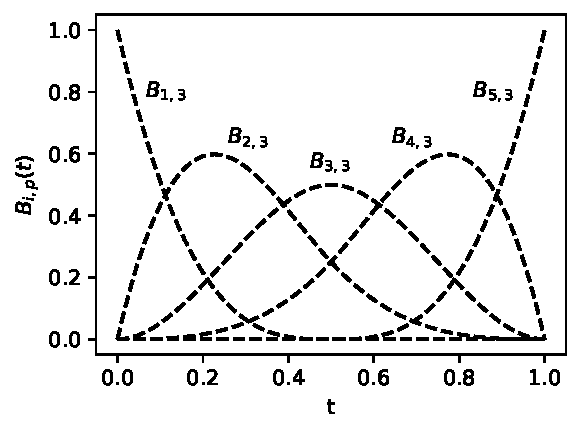
\includegraphics[width=\linewidth]{figures/MI estimation/B-spline basis functions - degree 3.pdf}
        \caption{}
        \label{subfig:B-spline fuctions}
    \end{subfigure}%
    ~
    \begin{subfigure}[t]{0.49\textwidth}
        \centering
        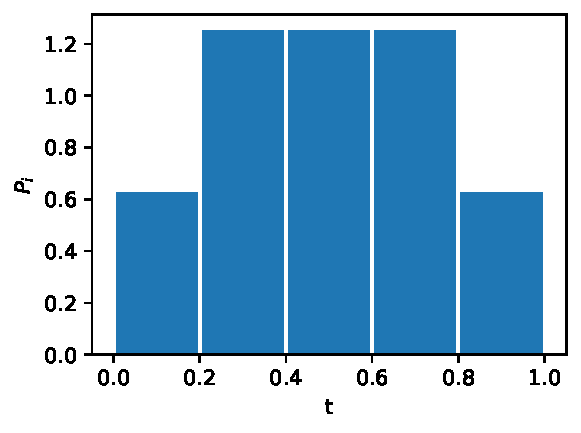
\includegraphics[width=\linewidth]{figures/MI estimation/B-spline marginal dist - degree 3.pdf}
        \caption{}
        \label{subfig:B-spline marginals}
    \end{subfigure}
    \caption{}
    \label{fig:B-splines}
\end{figure}
The fact that the B-splines sum to $1$ and that we have $m$ splines of degree $p$ is what we will use to estimate the density and in return the mutual information between two random variables based on observations. Namely, suppose we want to compute the mutual information, this can then be done by discretizing the random variables by binning. We assign the probability mass $P_{i,j}$ to bin $(i,j)\in \{1,\dots, m\} \times \{1,\dots, m\}$ as the fraction of observations in the domain corresponding to that bin. In particular, using Copula entropy, we would divide the unit interval into $m^2$ equal bins. As we saw earlier, in theory, increasing the number of bins will result in a more and more exact estimate of the mutual information. However, with limited observations, this is not the case as in the limit, the bins would not represent the true underlying distribution due to the finite number of observations. Namely, we would observe a few bins with $1$ observation and many with none. As an example, suppose we have $n$ observations and $m$ bins in both dimensions. Then, for $m$ large enough, $P_{i,j} = \frac{1}{n}$ for a hundred distinct bins as well as the marginal probability masses $P_i = \frac{1}{n}$ and $P_j = \frac{1}{n}$. But then,
\begin{align*}
    I\left(X_1^\Delta,X_2^\Delta\right) & = - \sum_{i=1}^{m} P_i \log P_i - \sum_{j=1}^{m} P_j \log P_j + \sum_{i,j = 1}^{m} P_{i,j} \log P_{i,j} \\
                                        & = - n \left(\frac{1}{n} \log \frac{1}{n}\right)                                                         \\
                                        & = \log n
\end{align*}
which is clearly independent of the true underlying distribution. However, if for each observation $x_j$ we assign it to bin $i$ with probability mass $B_{i,p}\left(x_j\right)$ this problem is mitigated to some extent as long as $m$ is not too large. It follows that in total each $x_j$ is assigned to all $m$ bins with a combined mass $1$ as $\sum_i B_{i,p} ( x_j ) = 1$. Thus, let $\left(\boldsymbol X^{(1)}, \boldsymbol X^{(2)}\right)$ be a pair of random vectors each of $d$ i.i.d variables representing observations drawn from a joint distribution, we then define the B-spline density estimator (i.e. a random variable) for $\boldsymbol X^{(1)}$ as 
$$P_{i}^{(1)} = \frac{1}{d} \sum_{j = 1}^{d} B_{i,p}\left(X_{j}^{(1)}\right), \quad i\in \{1,\dots, m\}$$
and similarly for $\boldsymbol X^{(2)}$. Furthermore, the B-spline joint density estimator is given by 
$$P_{i,j} = \frac{1}{d} \sum_{k= 1}^{m} B_{i,p}\left(X^{(1)}_k\right) \, B_{j,p}\left(X^{(2)}_k\right)$$
i.e. a product of the probability masses such that $\sum_{i,j = 1}^d P_{i,j} = 1$ and the marginal probability masses are given by $P_{i}^{(1)}$ and $P_{j}^{(2)}$ respectively.

However, there is still one problem. Namely, the marginals are not uniform when $p > 0$ when $\boldsymbol X^{(k)}$ is. This can also be seen from \autoref{subfig:B-spline marginals}. This is especially bad when computing Copula entropy as for e.g. a Gaussian random vector we would dramatically underestimate the mutual information as we shall also see in the next chapter. To see that this is the case, consider the expectation of $P_i^{(k)}$ for $k\in \{1,2\}$:
$$\mathbb{E}\left[P_i^{(k)}\right] = \frac{1}{d} \sum_{j = 1}^{d}\mathbb{E}\left[B_{i,p}\left(X_j^{(k)}\right)\right] = \int_{0}^{1} B_{i,p}\left(x\right)\, dx$$
Indeed, we would want this to be $\frac{1}{m}$ but from the Cox-deBoor recursion formula, we see that this is not the case. Namely, by choosing the knots as in \cite{RePEc:plo:pbio00:0050008} we see that the bins close to the boundary have too little probability mass. Thus, we turn our head to another family of splines called M-splines.


\subsection{M-splines}\label{subsec:M-plines - method}
Another known family of splines called M-splines have exactly the desired property of equal integrals. Namely, the M-splines $M_{i,p}$ all have unit integrals. Thus, rescaling with $\frac{1}{m}$ results in a family of splines $\tilde{M}_{i,p}$ such that on average we have that $P_i = \frac{1}{m}$. The M-splines equivalent to those of \autoref{fig:B-splines} are shown in \autoref{fig:M-splines}. Indeed, we see that the marginals are uniform. M-splines can similarly to B-splines by computed recursively by the following \cite{Monotone-Regression-Splines-in-Action}
\begin{align}
    M_{i,0}\left(t\right) & = \frac{1}{t_{i+1} - t_i}, \quad t\in [t_i, t_{i+1})                                                                                                                     \\
    M_{i,k}\left(t\right) & = \frac{k\left( \left(t - t_i\right) M_{i,k-1}\left(t\right) + \left(t_{i+k} - t\right) M_{i+1,k-1}\left(t\right)\right)}{\left(k-1\right) \left(t_{i+k} - t_{i}\right)}
\end{align}
However, now the problem is that the splines no longer sum to $1$ (after rescaling with $\frac{1}{n}$). Namely, we can no longer guarantee that the probability masses $P_{i,j}^M$ based on the M-spline sum to $1$. Thus, a renormalization is needed to ensure a proper probability mass function. From \autoref{fig:M-spline functions sum} we see that the effect of $\sum_{i = 1}^{m}\tilde{M}_{i,p}\left(x\right) \neq 1$ in this case is that observations on the interior are smoothed more than those near the boundary.
\begin{figure}[ht]
    \centering
    \begin{subfigure}[t]{0.49\textwidth}
        \centering
        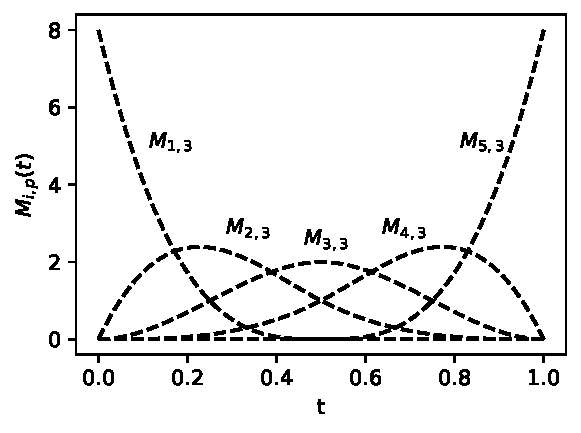
\includegraphics[width=\linewidth]{figures/MI estimation/M-spline basis functions - degree 3.pdf}
        \caption{}
        \label{subfig:M-spline functions}
    \end{subfigure}
    \hfill
    \begin{subfigure}[t]{0.49\textwidth}
        \centering
        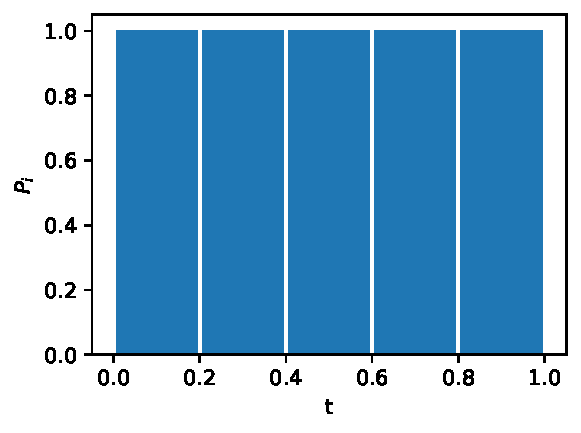
\includegraphics[width=\linewidth]{figures/MI estimation/M-spline marginal dist - degree 3.pdf}
        \caption{}
    \end{subfigure}
    \caption{$P_i$ is area of each rectangle i.e. $0.2$.}
    \label{fig:M-splines}
\end{figure}

This can however be a useful property especially for a bivariate Gaussian for which the Copula density, as we shall see, have peaks at $(0,0)$ and $(1,1)$ while being relatively smooth elsewhere.

We note that through construction, one can create a family of splines that both sum to 1 have integrals $\frac{1}{m}$. However, as these spline-based smoothing methods does not perform well in general perform very differently for different $m$ with the lack of continuously varying this parameter that acts as a regularizing parameter, as we shall see in \autoref{chap:results}, we only present the method for constructing such splines in \autoref{sec:A family of better splines for Copula entropy estimation} and instead consider a more general way of estimating the Copula density, namely kernel density estimators.

\begin{figure}[ht]
    \centering
    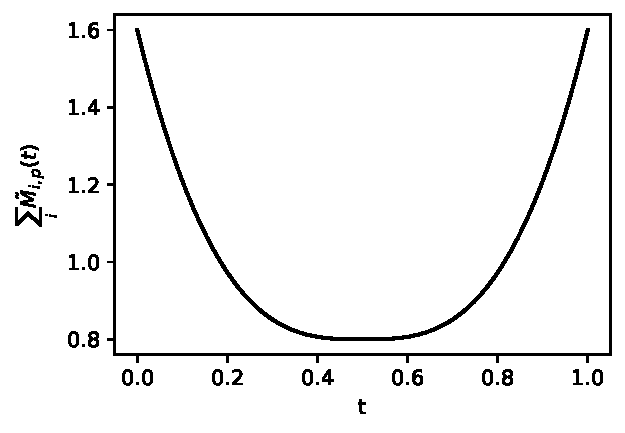
\includegraphics[width = .55\linewidth]{figures/MI estimation/M-spline coefficient sum - degree 3.pdf}
    \caption{}
    \label{fig:M-spline functions sum}
\end{figure}

% \cite{Monotone-Regression-Splines-in-Action} a set of $n$ basis functions indexed by $i$. Letting the order of the basis function equal $p+1$ such that the basis functions are polynomials of degree p. Define knots to be $t_1 = \dots = t_k = 0$ and $t_{n+1} = \dots = t_{n+k} = 1$. furthermore, we choose the remaining $n-k$ (interior) knots to be equally distributed on $[0,1]$ i.e. if $3$ interior points, they are $1/4$, $1/2$ and $3/4$ respectively. (slightly reformualted to agree with the notation for B splines)








\newpage
\subsection{Naïve KDE}
As we shall see in \autoref{subsec:Spline and KDE based CE estimation}, if one can accurately determine the Copula density of $X_1$ and $X_2$, then using an approximation of the integral, one can calculate the mutual information to any precision wanted. This clearly follows from the above analysis regarding the behavior of the discretization of $X_1$ and $X_2$ in the limit as the mesh gets more fine. Thus, if we can estimate the joint Copula density well, we obtain a good estimate of the mutual information of $X_1$ and $X_2$. A widely used non-parametric method for density estimation is kernel density estimation. Namely, if $\{{\boldsymbol x}_i\}$ is a set of $n$, $d$-dimensional observations from a population, i.e. $\boldsymbol x_i$ can be both scalars and vectors in the case of a multidimensional distribution, the kernel density estimator (KDE) of the probability density function is in general given as
\begin{equation}\label{eq:KDE definition}
    \hat{f}(\boldsymbol x) = \frac{1}{n}\sum_{i=1}^n \frac{1}{\prod_{j= 1}^d \boldsymbol h_{i,j}} K\left(\frac{\boldsymbol x-\boldsymbol x_i}{\boldsymbol h_i}\right)
\end{equation}
where $\boldsymbol h_i$ is the bandwidth (vector) associated with observation $\boldsymbol x_i$ and $K$ is the kernel (function), defined on the domain of $\boldsymbol X$ which is often $\mathbb{R}^d$. Often, the bandwidths $\boldsymbol h_i$ are taken to be equal and initially, we shall do so as well. Furthermore, the kernel $K$ is a non-negative function, and is in itself a density function i.e. integrates to $1$ as shown below. This ensures that $\hat{f}$ in \autoref{eq:KDE definition} integrates to $1$ and is non-negative i.e. a proper distribution.
$$\int_{\mathbb{R}^d} K(\boldsymbol x) \, d\boldsymbol x = 1$$
In one dimension, a particular useful kernel is the Gaussian kernel given by $K(x) = \phi\left(x\right)$ where $\phi$ is the density function for the standard Normal distribution. $\phi$ is chosen due to its simple behavior and mathematical properties. In particular, we shall see in the following section, that the properties of the Gaussian kernel allows for simple expressions when correcting for a boundary such that computation is quick and efficient. For multiple dimensions, we often consider product kernels, which are kernels $K$ of the form
\begin{equation}\label{eq:product kernel}
    K\left(\boldsymbol x\right) = \prod_{i = 1}^{d} K_i\left(x_i\right)
\end{equation}
I.e. just a product of kernels. In particular, we choose $K_i = \phi$ again due to the numerical properties. Thus, initially, we have a KDE $\hat{f}$ of the following form where we once again note that $\boldsymbol h_i = \boldsymbol h$ for all $i\in \{1,\dots, n\}$ such that $h_j$ denotes the bandwidth associated with the $j$th dimension.
$$\hat{f}\left(\boldsymbol x\right) = \frac{1}{n\prod_{j = 1}^{d}h_j} \sum_{i=1}^n \prod_{j = 1}^{d} \phi \left(\frac{x_j - x_{i,j}}{h_j}\right)$$



The choice of bandwidth $\boldsymbol h$ is important regarding a trade-off between the variance and bias of the KDE. In general, we want to choose $h$ as small as possible resulting in the least bias but a too small $\boldsymbol h$ will result in large variance of the estimator. In particular, $\boldsymbol h$ acts as a smoothing parameter like the number of bins from the previous section, but here, we can choose any $h > 0$ making the KDE a much more versatile tool. Often the \textit{Mean Integrated Square Error} (MISE) is used which is the expected $L^2$-norm of $\hat{f} - f$ i.e.
$$\text{MISE} \left(\hat{f}\right) = \mathbb{E}_{f} \left[\int_{\mathbb{R}^d} \left| \hat{f}\left(\boldsymbol x\right) - f\left(\boldsymbol x\right)\right|^2 \, d\boldsymbol x\right] $$
which of course depends on $\boldsymbol h$. The expectation $\mathbb{E}_f$ denotes the expectation with respect to the samples $\{\boldsymbol x_i\}$ of $\boldsymbol X$ with (true) density distribution function $f$. Expanding the above expression, we obtain a simple expression relating MISE to the integrated squared bias and integrated variance as shown below
$$\text{MISE} \left(\hat{f}\right) =  \int_{\mathbb{R}^d} \left| \mathbb{E}_{f}\left[\hat{f}\left(\boldsymbol x\right)\right] - f\left(\boldsymbol x\right)\right|^2 \, d\boldsymbol x  +  \int_{\mathbb{R}^d} \text{Var} \left[ \hat{f}\left(\boldsymbol x\right)\right] \, d\boldsymbol x$$
It is however quite complicated to optimize the above, and we shall thus often use a simple rule of thumb known as Scott's rule \cite{Scott1992MultivariateDE} for choosing $\boldsymbol h$. Namely, for product kernels, we let the bandwidths of each dimension $j$ equal the following where $\hat{\sigma}_j$ is the standard deviation estimated from the observations of $X_j$
$$h_{j}^{Scott} = \hat{\sigma}_j n^{-1/(d+4)}, \quad j \in \{1,\dots, d\}$$

\begin{figure}[ht]
    \centering
    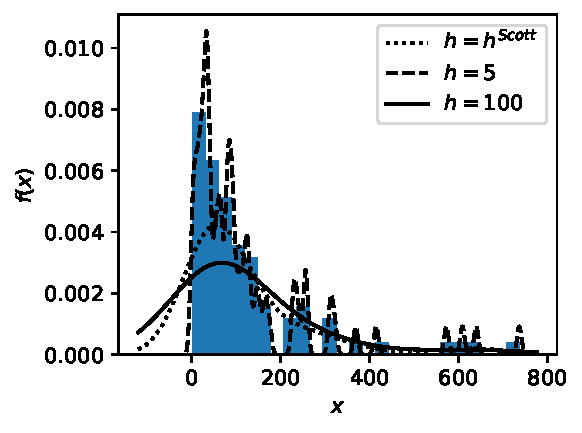
\includegraphics[width = .6\linewidth]{figures/MI estimation/suicide data example.pdf}
    \caption{The suicide data from MHE. The $86$ observations are shown as a histogram of densities along with Gaussian KDEs with bandwidth $h=5$ and $h=100$ and $h$ chosen from Scott's rule $h = \hat{\sigma} n^{-1/5} \approx 59.86$.}
    \label{fig:suicide KDE example}
\end{figure}

In \autoref{fig:suicide KDE example}, we have shown a basic example in one dimension with two different manual choices of the bandwidth $h$ and $h$ chosen by Scott's rule. We have used data from \cite{Density-Estimation-and-Suicide-Risks-in-Psychiatric-Treatment}, tabulated in \cite{Silverman86} which has been used in \cite{Jones1993SimpleBC} which propose a method for correcting the KDE near a boundary which we shall discuss in the following section. The data consists of $86$ observations regarding suicide and is known to be non-negative. In consideration of the reader, we have included the observations in \autoref{tab:suicide data}. It is clear that using $h^{Scott}$ results in what we qualitatively would deem a good estimate for the probability density function as $h = 100$ seen to be overly smoothed whereas $h = 100$ too under-smoothed. In particular, from repeated samples we would expect the estimator using $h= 100$ would have large bias but small variance whereas for $h = 5$ would have much larger variance but smaller bias. However, a problem the estimators, $h = 100$ and $h = h^{Scott}$ especially, have is that they have probability mass below $0$ which in this case is unwanted. I.e. when restricting $\hat{f}$ to $[0,\infty)$ they are no longer proper probability distribution functions as they do not integrate to $1$. A Simple fix could be to simply rescale $\hat{f}$ such that this is the case, but as seen from the example in \autoref{fig:suicide KDE example - rescaled} where this method is applied to the same example as above, this tends to underestimate the peaks especially near the boundary.

\begin{figure}[ht]
    \centering
    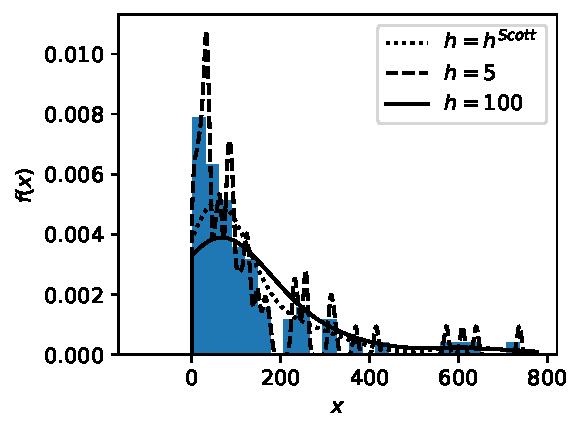
\includegraphics[width = .6\linewidth]{figures/MI estimation/suicide data example - rescaled.pdf}
    \caption{Using a rescaled version of $\hat{f}$ on the interval $[0,\infty)$ and disregarding any probability mass below $x=0$ we obtain proper probability distributions once again. However, neither of the methods capture the peak near the boundary $x=0$. In particular, although $h^{Scott}$ still seem to be a good choice for $h$, the KDE does not capture the tendency observed in the data.}
    \label{fig:suicide KDE example - rescaled}
\end{figure}

We note that using a non-constant $h$ would improve on this behavior, but simpler methods exists, and we thus proceed in the next section with a method that shows great promise regarding this seemingly fundamental issue with KDE. In particular, we refer to a systematic way of letting the shape of each of the kernels depend on the associated observation $x_i$.


\newpage
\subsection{Boundary Corrected KDE}\label{sec:Boundary corrected KDE}
Before introducing the boundary corrected kernels presented by \cite{Jones1993SimpleBC}, we mention another simple method of boundary correction called reflection. Namely, suppose without loss of generality $x = 0$ is the lower boundary of the domain of $\boldsymbol X$ and let $\hat{f}$ be KDE as from the previous section. Then, the reflection boundary corrected KDE denoted $\hat{f}_R$ is defined as
$$\hat{f}_R(x) = \hat{f}(x) + \hat{f}(-x)$$
Clearly, $\hat{f}_R$ is non-negative, and it follows from the below that it is also a proper density function as the probability mass is $1$
$$\int_{0}^{\infty} \hat{f}_R \left(x\right) \, dx = \int_{0}^{\infty} \hat{f} \left(x\right) + \hat{f} \left(-x\right) \, dx = \int_{0}^{\infty} \hat{f} \left(x\right) + \int_{-\infty}^{0}\hat{f} \left(x\right) \, dx = 1$$
Also, the above is easily extended to two boundaries. Namely, if the domain is $[a,b]$, the reflection boundary corrected KDE is given by
$$\hat{f}_R\left(x\right) = \hat{f}\left(x\right) + \hat{f}\left(2a-x\right) + \hat{f}\left(2b-x\right),\quad x \in [a,b]$$
If we once again apply this to the suicide data, comparing to \autoref{fig:suicide KDE example - rescaled} we see a big improvement near the boundary as shown in \autoref{fig:suicide KDE example - reflected}. However, we still proceed with the method originally presented in \cite{Jones1993SimpleBC}. The reason for this is that when testing for distribution type using the Kolmogorov Smirnov test (on a $5\%$ significance level) we reject that the observations originate from $\hat{f}_R$ with $h = 100$.
\begin{figure}[ht]
    \centering
    \begin{subfigure}[t]{0.49\linewidth}
        \centering
        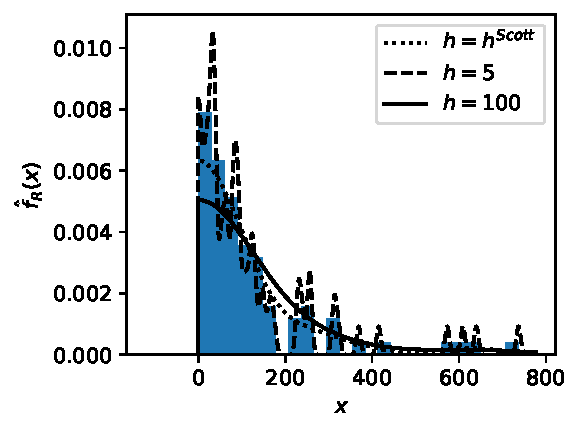
\includegraphics[width = \linewidth]{figures/MI estimation/suicide data example - reflection.pdf}
        \caption{}
        \label{fig:suicide KDE example - reflected}
    \end{subfigure}
    \hfill
    \begin{subfigure}[t]{0.49\linewidth}
        \centering
        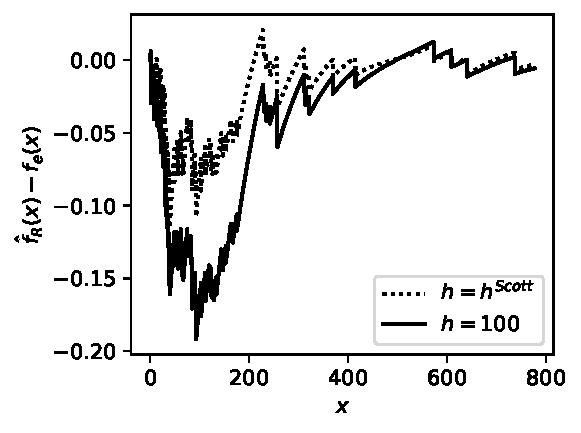
\includegraphics[width = \linewidth]{figures/MI estimation/suicide data example - reflection - Kolmogorov Smirnov.pdf}
        \caption{}
        \label{fig:Kolmogorov Smirnov DN}
    \end{subfigure}
    \caption{}
\end{figure}
For $h=5$ we do not but due to the above considerations regarding the integrated point wise variance of the estimator, this choice of $h$ is undesired in either case. For $h = h^{Scott}$ we do not reject the distribution but as the shape of the error resembles the error for $h=100$ we suspect that there is some systematic error which we also see from \autoref{fig:Kolmogorov Smirnov DN}. Furthermore, the largest deviation from the empirical distribution to $\hat{f}_R$ is close to the boundary (as expected). The test statistics (the largest absolute difference $D$ between the distribution functions and the adjusted statistic) is shown in \autoref{tab:relfection Kolmogorov Smirnov} where the adjusted test statistic should be compared to the critical value $1.358$ on a $5\%$ significance level. Furthermore, to really test the kernel density estimators, one should compute the MISE based on bootstrap and/or cross-validation. In particular, this way larger $h$ i.e. more smoothing would be more favorable compared to the Kolmogorov Smirnov test results which shows small $h$ best represent the empirical distribution.
\begin{table}[ht]
    \centering
    \begin{tabular}{l|rr}
        $h$         & $D$        & Adjusted $D$ \\\hline
        $5$         & $0.029042$ & $0.27315$    \\
        $h^{Scott}$ & $0.11262$  & $1.0593$     \\
        $100$       & $0.19194$  & $1.8053$
    \end{tabular}
    \caption{$\left(\sqrt{n} + 0.12 + 0.11/\sqrt{n}\right) D$}
    \label{tab:relfection Kolmogorov Smirnov}
\end{table}
% \cite{Jones1993SimpleBC} also shows that the error the method of reflection  $\mathbb{E}\left[\right]$

We now turn our attention to the boundary corrected KDE from \cite{Jones1993SimpleBC}. They shortly described this in \cite{Nonparametric-copula-entropy-and-network-deconvolution-method-for-causal-discovery-in-complex-manufacturing-systems} where it was used to estimate the mutual information in terms of Copula entropy. However, issues arise when using this KDE in terms of non-negativity of the KDE and the facts that it does not integrate to unity. All of these issues can however be handled in a general way without effecting the results regarding bias of the estimator as we shall also see from the above example on suicide data. In particular, \cite{Jones1993SimpleBC} show that the bias of their estimator $\hat{f}_L$ is of order $\mathcal{O}\left(h^2\right)$ whereas the reflection method discussed above has $\mathcal{O}\left(h\right)$ bias. The basic idea of $\hat{f}_L$ is that it is a linear combination of a symmetric kernel $K$ and $x \, K$ i.e. a first order kernel. They do however only give explicit expressions when a lower bound at $x = 0$ is enforced but the math generalize nicely to $2$ boundaries. In particular, we shall let $x_u$ denote the upper bound of the domain and keep $x= 0$ as the lower bound. Before continuing with the derivation and results regarding implementation for the Gaussian kernel we note that in \texttt{R}\footnote{https://search.r-project.org/CRAN/refmans/evmix/html/bckden.html}, there is a library \texttt{evmix} which implements the boundary corrected KDE from \cite{Jones1993SimpleBC} but only for $1$ dimension and only with a lower bound at $x=0$. We thus expand on this library (although in \texttt{Python}) to include both lower and upper bounds and furthermore, generalize to multiple dimensions using a product kernel as noted in \autoref{eq:product kernel}.

To expand on the boundary corrected KDE to include an upper bound on the domain, we define the functions $a_m\left(x\right)$. Note that in \cite{Jones1993SimpleBC}, they define $a_m$ as a function of $p = x / h$ where $h$ is the bandwidth, but to keep the expression later on easier to understand in terms of kernel centers etc. we instead define them as a function of $x \in [0,x_u]$. The reason for initially defining $a_m$ in terms of $h$ is to keep the bandwidth out of the expression, which we then define as follows, when there is no upper bound
$$a_m\left(x\right) = \int_{-\infty}^{\frac{x}{h}} u^m K\left(u\right) \, du, \quad x\in [0,\infty)$$
The above is actually equal to the part of the $m$th moment of the kernel centered at $x$ (and width bandwidth $h$), that is inside the interval $[0,\infty)$ up to a difference in sign. In particular, using the change of variables $z=x-hu$ we have that
$$a_m\left(x\right) = \left(-1\right)^m  \int_{0}^{\infty} \left(\frac{z-x}{h}\right)^m \, \frac{1}{h}K\left(\frac{z-x}{h}\right) \, dz$$
where we have used that $K$ assumed to be symmetric. Indeed, the above is as described the part of the $m$th moment that comes from $[0,\infty)$ (up to a difference in sign) of the kernel that is centered at $x$ with bandwidth $h$. From this, it is a natural extension to replace the upper bound of the integral with $x_u$ which, when expanding on the initial definition in \cite{Jones1993SimpleBC} as done in e.g.
\cite{Simple_and_eff_boundary_correction_for_kern_densities}
turns out to be the correct adjustment. Thus, $a_m$ can be understood as part of the moments which we shall then use as normalizing functions. Thus, for an upper bound $x_u$ we find that instead $a_m$ is defined as
$$a_m\left(x\right) = \int_{\frac{x-x_u}{h}}^{\frac{x}{h}} u^m K\left(u\right)\, du, \quad x\in [0,x_u]$$
The boundary adjusted KDE which we shall denote $K^L$ and index depending on the $i$th kernel center is then given by
\begin{equation}\label{eq:jones bc corrected kernel}
    K_i^{L} \left(x\right) = \frac{1}{h}\frac{a_2\left(x\right) - a_1\left(x\right) \frac{x - x_i}{h}}{a_0 \left(x\right) a_2\left(x\right) - a_1^2 \left(x\right) } \, K\left(\frac{x - x_i}{h}\right)
\end{equation}
For the Gaussian kernel, $a_m\left(x\right)$ for $m \in \{0,1,2\}$ are easily computed and implemented in code through standard routines as they have simple closed forms in terms of $\phi$ and $\Phi$, i.e. the standard Gaussian density and distribution functions. Namely, for $a_0$ we simply have that by definition of $\Phi$
\begin{align*}
    a_0\left(x\right) & = \int_{\frac{x-x_u}{h}}^{\frac{x}{h}} \phi(u) \, du              \\
                      & = \Phi\left(\frac{x}{h}\right) - \Phi\left(\frac{x-x_u}{h}\right)
\end{align*}
And similarly, for $a_1$, using that $\int u \,\phi \left(u\right) \, du = - \phi\left(u\right) + C$
\begin{align*}
    a_1\left(x\right) & = \int_{\frac{x-x_u}{h}}^{\frac{x}{h}} u \phi(u) \, du           \\
                      & = \phi \left(\frac{x-x_u}{h}\right)-\phi\left(\frac{x}{h}\right)
\end{align*}
Finally, for $a_2$ we have, using integration by parts for the first step
\begin{align*}
    a_2\left(x\right) & = \int_{\frac{x-x_u}{h}}^{\frac{x}{h}} u^2 \phi(u) \, du                                                                                                                                    \\
                      & = \left[- u \phi \left(u\right)\right]_{\frac{x-x_u}{h}}^{\frac{x}{h}} + \int_{\frac{x-x_u}{h}}^{\frac{x}{h}} \phi \left(u\right) \, du                                                     \\
                      & = \left(\frac{x-x_u}{h} \phi\left(\frac{x - x_u}{h}\right) - \frac{x}{h} \phi\left(\frac{x}{h}\right)\right) + \left(\Phi\left(\frac{x}{h}\right) - \Phi\left(\frac{x-x_u}{h}\right)\right) \\
                      & = \frac{x}{h} a_1\left(x\right) - \frac{x_u}{h} \phi \left(\frac{x - x_u}{h}\right) + a_0\left(x\right)
\end{align*}
From the improved bias of $\mathcal{O} \left(h^2\right)$ for $K_i^L$, we have then obtained an estimator that should perform better in terms of a smaller MISE as we have less bias and by choosing $h$ optimally, we should expect small variance as well. \autoref{fig:suicide KDE example - jones1993} shows the KDE $\hat{f}_L$ using $K^L$ as the kernel (with $x_u = \infty$) and is compared to the reflected kernel from above using the same bandwidth. We note that $\hat{f}_L$ has be rescaled such that it integrates to unity on $[0,\infty)$. Also, from \autoref{fig:Kolmogorov Smirnov DN - jones1993} we see that the density is not statistically significant, and although we can not conclude from this alone, we observe that the deviation from the empirical distribution functions is less than that of the reflected KDE.

As noted above, we need to rescale $\hat{f}_L$ to unity as the kernels in \autoref{eq:jones bc corrected kernel} does not have unit integrals. Furthermore, $\hat{f}_L$ is not even ensured to be non-negative. This can be handled in multiple ways. One way is to simply take the maximum of $\hat{f}_L$ and $0$ effectively cutting off any negative density however in \cite{A-simple-nonnegative-boundary-correction-method-for-kernel-density-estimation}, a method is given for KDE based on $K_i^L$ specifically, ensuring the $\mathcal{O}\left(h^2\right)$ bias of the estimator. Namely, let $K^N_i$ be given as
$$K^N_i \left(x\right) = \frac{1}{h\,a_0\left(x\right)} K\left(\frac{x-x_i}{h}\right)$$
which is then the kernel, locally renormalized using $a_0$. We then define the related KDE as
$$\hat{f}_N \left(x\right) = \frac{1}{n} \sum_{i = 1}^{n} K_i^N \left(x\right)$$
which is then non-negative everywhere as $a_0\left(x\right), K\left(x\right) > 0$. The non-negative boundary corrected KDE, denoted $\hat{f}_P \left(x\right)$ is then defined as
$$\hat{f}_P \left(x\right) =\hat{f}_N \left(x\right) \, e ^{\frac{\hat{f}_L \left(x\right)}{\hat{f}_N \left(x\right)} - 1} $$
This $\hat{f}_P$ is also shown in \autoref{fig:suicide KDE example - jones1993 - total figure} resulting in identical density functions. We note that $\hat{f}_P$ works by multiplying the non-negative $\hat{f}_N$ by a (large positive) constant when $\hat{f}_L$ is larger than $\hat{f}_N$ and thus drives $\hat{f}_N$ towards $\hat{f}_L$. However, from implementation and trying on different distributions, sometimes we observe some odd behavior that can easily be derived from the definition of $\hat{f}_P$. Thus, we propose a modification to overcome these odd properties of $\hat{f}_P$. Namely, suppose both $\hat{f}_L$ and $\hat{f}_N$ are close to $0$ at some point $x$. If $\hat{f}_L$ is a magnitude of $10$ larger than $\hat{f}_N$, then $\hat{f}_P$ is approximately $8000 \cdot \hat{f}_N$ which even if $\hat{f}_N$ is small may be large. Thus, it is possible even if both  are close to $0$, that $\hat{f}_P >> 0$ which is in contrast to what we would want from the estimator. Thus, we propose a regularized KDE version of $\hat{f}_P$ denoted $\hat{f}_{regP}$ which is obtained from first rewriting $\hat{f}_P$ as follows
$$\hat{f}_P\left(x\right) = \bar{f}\left(x\right) \, e^{\frac{\tilde{f}\left(x\right) - \hat{f}\left(x\right)}{\hat{f}\left(x\right)} }$$
then, we introduce the regularizing parameters $\lambda \geq 0$ such that
$$\hat{f}_{regP}\left(x\right) = \bar{f}\left(x\right) \, e^{\frac{\tilde{f}\left(x\right) - \hat{f}\left(x\right)}{\hat{f}\left(x\right) + \lambda} }$$
In practice, we have found that $\lambda = 0.001$ is a sufficient regularization whilst preserving the shape. A small $\lambda$ is preferred as then we are ensured $\mathcal{O}\left(h^2\right)$ behavior of the bias. In \autoref{fig:suicide KDE example - jones1993 - total figure} we have also shown this regularized version with $\lambda = 0.001$ and observe that it is basically identical to $\hat{f}_P$ on the domain while also behaving well numerically for large $x$, where the issue discussed above arise for $\hat{f}_P$.
\begin{figure}[ht]
    \centering
    \begin{subfigure}[t]{0.49\linewidth}
        \centering
        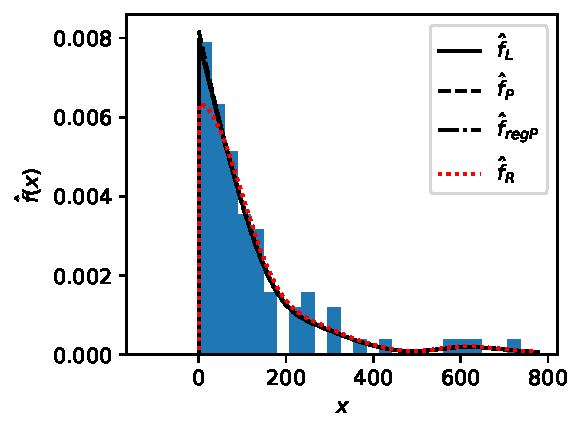
\includegraphics[width = \linewidth]{figures/MI estimation/suicide data example - Jones1993.pdf}
        \caption{}
        \label{fig:suicide KDE example - jones1993}
    \end{subfigure}
    \hfill
    \begin{subfigure}[t]{0.49\linewidth}
        \centering
        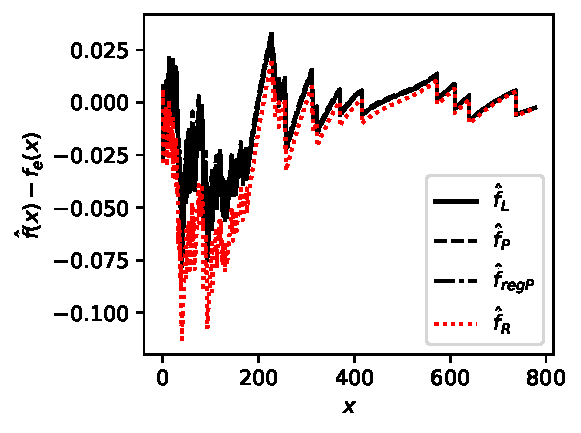
\includegraphics[width = \linewidth]{figures/MI estimation/suicide data example - Jones1993 - Kolmogorov Smirnov.pdf}
        \caption{}
        \label{fig:Kolmogorov Smirnov DN - jones1993}
    \end{subfigure}
    \caption{}
    \label{fig:suicide KDE example - jones1993 - total figure}
\end{figure}
Before continuing with a few more interesting methods of density estimation and mutual information estimation in particular, we note that in the same \texttt{R} package there is a KDE based on the Gaussian Copula density which at first glance might seem a good choice especially if we are trying to estimate the density of a Copula that we know to be Gaussian. The KDE is based on \cite{Kernel-Type-Density-Estimation-on-the-Unit-Interval}, and trivially we get that the domain of the basis functions is already $[0,1]$. In particular, the kernel for a given bandwidth $h$ and kernel center $x_i$ is given by
$$K^{GC}_i \left(x\right) = \frac{1}{h \sqrt{2-h^2}} e^{-\frac{\left(1 - h^2\right)}{2 h^2 \left(2-h^2\right)} \left( \left(1 - h^2\right) \left(\left(\Phi^{-1} \left(x\right)\right)^2 + \left(\Phi^{-1} \left(x_i\right)\right)^2 \right) - 2 \Phi^{-1} \left(x\right) \, \phi^{-1}\left(x_i\right) \right) }$$
which is obtained by letting $h^2 = 1-\rho$ in the original expression for the Gaussian Copula density. However, in practice, we shall see that this choice of kernel has some numerical instabilities especially for large correlations i.e. small $h$ and does not perform as well as $\hat{f}_{regP}$ even when using their optimal bandwidth.

Furthermore, we note that as observations are initially transformed such that they are approximately uniform on $[0,1]$, the variance of these uniform observations $u_i = \hat{F}\left(x_i\right)$ will also be approximately $1/12$ and hence the Scott rule of thumb will give a near constant bandwidth. However, as we shall see later, the performance is drastically improved by choosing smaller bandwidth for subdomains with high density. We thus note that a local bandwidth should be considered in the future. This could e.g. by using $k$-nearest neighbor and the distances of these which is the basic idea of \cite{Estimating-mutual-information-Kraskov}. Although we will not be using this method as it is out of scope for this paper, we note that their estimator seem to result in good estimates when $n \geq 300$. Using the core ideas of this paper, one could perhaps deduce a better algorithm for choosing $h$ globally or locally.

Finally, we note that a recent method based on diffusion \cite{A-Novel-Nonparametric-Density-Estimator} \cite{Kernel-density-estimation-via-diffusion} which shows great potential. Without going into too much detail, it works by considering the following PDE
$$\frac{\partial}{\partial t} \hat{f}\left(x;t\right) = \frac{1}{2} \frac{\partial^2}{\partial x^2} \hat{f}\left(x;t\right)$$
where $t = h^2$. The Gaussian kernel is then the unique solution when the domain is $\mathbb{R}$ with condition $\hat{f}\left[x;0\right] = \frac{1}{n} \sum_{i=1}^{n} \delta \left(x-x_i\right)$ i.e. the observations is the boundary condition at $h=0$. If instead we add that the support should be e.g. $[0,1]$ the Neumann boundary conditions on the boundary results in an analytical solution. Namely, from the boundary conditions
$$\frac{\partial}{\partial x} \hat{f}\left(x;t\right) \bigg\rvert_{x = 0} = \frac{\partial}{\partial x} \hat{f}\left(x;t\right) \bigg\rvert_{x = 1} = 0$$
the analytical solution to $\hat{f}$ is
$$\hat{f}_D\left(x ; t\right) = \frac{1}{n} \sum_{i=1}^{n} K_i^D \left(x\right)$$
where
$$K_i^D \left(x\right) = \frac{1}{h}\sum_{k=-\infty}^{\infty} \phi\left(\frac{x - \left(2k+x_i\right)}{h}\right) + \phi\left(\frac{x - \left(2k-x_i\right)}{h}\right)$$
which is similar to the reflection method from above. They even give an algorithm for calculating $t$ which from the example below appear to work very well. Before presenting this example we note that although it is out of scope to use this method in the following chapter, it would be interesting to see how well it would perform as it is the only KDE here that does not use any transformation near the boundary while still being consistent at the boundary as they show in \cite{Kernel-density-estimation-via-diffusion}.

\begin{example}[Diffusion based KDE]
    Let $X\sim \text{Beta} \left(1,4\right)$ such that $f(x) = 4 \left(1- x\right)^3$ for $x\in \left[0,1\right]$ and thus $F\left(x\right) = 1 - (1-x)^4$. Generating $1000$ samples from the distribution and using the algorithm in \cite{Kernel-density-estimation-via-diffusion} to estimate the bandwidth, we get a bandwidth $h^D = 0.05461$ whereas with Scott's rule we get $h ^{Scott} = 0.04145$. From \autoref{fig:beta dsitribution example} we see that diffusion and the regularized boundary corrected KDE $\hat{f}_{regP}$ from above agree almost everywhere. Only near the lower boundary at $x=0$ there is a significant difference and here $\hat{f}_{regP}$ seem to fit the true distribution better. This is due to the Neumann boundary condition which enforce $\hat{f}_D$ to have horizontal derivative at both boundaries. Note that we have used both the $h^D$ and $h^{Scott}$ bandwidth for the regularized boundary corrected KDE resulting in basically no difference.

    \begin{figure}[ht]
        \centering
        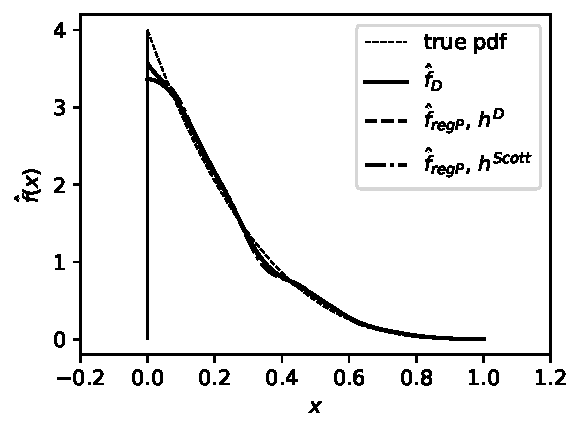
\includegraphics[width = .7\linewidth]{figures/MI estimation/beta dist example - comparison with diffusion and jones.pdf}
        \caption{Using the diffusion based KDE on $1000$ samples from a $\text{Beta}\left(1,4\right)$ distribution, we see that in general it fits very well. Only at the boundary $x=0$ there seems to be a problem which on the other hand, $\hat{f}_{regP}$ does not seem to suffer from to the same extend. In particular, repeating the experiment, $\hat{f}_{regP}$ is on average $4$ at $x = 0$ while $\hat{f}_{D}$ constantly seem to undershoot.}
        \label{fig:beta dsitribution example}
    \end{figure}
\end{example}
At this point, we thus have a complete set of methods for both estimating the mutual information from observations and from these, algorithms to estimate the (causal) structure depending on assumptions regarding direction i.e. a topological ordering of the variables. We thus proceed with numerical results in the following chapter and apply the framework on both fully controlled systems and the observations from \autoref{chap:data}.


\end{document}








% \newpage

% vi har nu vores endelig KDE, men i R var der også en copula function som så interessant ud. kernel er så bare gaussian copula. 


% Also, in R we see a copula method which is a $[0,1]$ domain method using gaussian copula as kernel such that it is reflexive in x and kernel point Xi. Could also be used and we have implemented this as the above using the products of kernel. \cite{Kernel-Type-Density-Estimation-on-the-Unit-Interval}

% Vi kan dog i resultater se at den ikke performer specialet godt, også selvom man bruger deres "optimerede" bandwidth.



% Vi ser senere i resultater at bandwidth er stort set ens da var 1/12 (uniform). Og for høje correlation, kan det betale sig at sætte lav bandwidth. 

% We shall see that for a pre-fixed bandwidth, we obtain an error around $0.2$ and as we shall see, adjusting the bandwidth corrects this. However, to make the framework more self-drive, we hence have the need for a more general scheme of choosing the optimal kernel (locally)




% Så en adaptive metode til at bestemme lokale bandwidth ville være godt. En metode der minder om er:


% In \cite{Estimating-mutual-information-Kraskov} they propose an approach using k-nearest neighbours which appear to give good results for $N \geq 300$. Using some of the core ideas from this paper, one could perhaps deduce a better non-global estimator of $h$. They show that they have in general better performance for estimating $I$ which we have not dived into, but comparing their results to what we shall later observe from our own implementations, theirs are very good and accurate and from more than 300 observations, $\rho = 0.9$ should be estimated within $0.01$ according to their figure 2 where we also observe a general trend that the larger the correlations is and thus information, the larger the error which is to be expected as almost identical correlation can have vastly different mutual information for large enough $\rho$.



% Dog, eksisterer følgende artikel hvor lokal bandwidth bruges. \cite{A-Novel-Nonparametric-Density-Estimator}. Dog ved at oversætte deres kode fandt vi at bandwidth skulle regulariseres mere (så generelt større), men vi har valgt ikke at fotsætte med dette, dog nævne fordi kunne være smart ift. problem med ikke lokal bandwidth for ovenstående

% Samme forfatter har også (senere), med en anden lavet density estimator ud fra diffusion og givet algoritme. Der er bandwidth dog konstant, men mulighed for at den kunne performe bedre. Vi nævner et kort eksempel, hvor vi viser styrken ved algoritmen, som helt selv finder en god h (ud fra MISE)






% \subsection{Diffusion based KDE}
% \cite{Kernel-density-estimation-via-diffusion} shows great promise also, we have implemented this in python as well but have chosen to focus on the above methods as time did not permit the exploration of this method further. However, we shall later see some results on this algorithm that shows why this method should be investigated further and hence why it is mentioned here

% The very big advantage and selling point for this method is that it does not use any transform or boundary correction except for the Neumann boundary conditions


% Sample from beta density given by $4 \left(1- x\right)^3$ for $x\in \left[0,1\right]$ such that $F(x) = 1 - (1-x)^4$ and hence we can sample from this using e.g. $X = 1 - (1-U)^{1/4}$



% The adaptive kernel density estimator also works ok, but in this context it seems to be having too small bandwidths. It works using a regularized EM algorithm but again, due to limit of time, we did not pursue this further although choosing how much the bandwidth is regularized or penalizing the integral of the absolute second order derivative would likely improve the results.